\title{データ分析教育へのアクティブラーニング手法の導入提案と実践}
\author{プロジェクトマネジメントコース\\
ソフトウェア開発管理グループ\\
矢吹研究室\\
1342015\\
板倉啓太}
\date{}
\begin{document}
\maketitle

%本テンプレートの余白は,卒論マニュアルで指示されたものとは違っているが,1ページあたりの文字数は40文字x40行と,卒論マニュアル通りになっている。文字間隔や行間隔を調整して,余白をマニュアル通りにすることもできるが,それでは文章が読みにくくなるため,このような対応をしている。

%\noindent
□□□□□□□□□■□□□□□□□□□■□□□□□□□□□■□□□□□□□□□■
□□□□□□□□□■□□□□□□□□□■□□□□□□□□□■□□□□□□□□□■
□□□□□□□□□■□□□□□□□□□■□□□□□□□□□■□□□□□□□□□■
□□□□□□□□□■□□□□□□□□□■□□□□□□□□□■□□□□□□□□□■
□□□□□□□□□■□□□□□□□□□■□□□□□□□□□■□□□□□□□□□■
□□□□□□□□□■□□□□□□□□□■□□□□□□□□□■□□□□□□□□□■
□□□□□□□□□■□□□□□□□□□■□□□□□□□□□■□□□□□□□□□■
□□□□□□□□□■□□□□□□□□□■□□□□□□□□□■□□□□□□□□□■
□□□□□□□□□■□□□□□□□□□■□□□□□□□□□■□□□□□□□□□■
□□□□□□□□□■□□□□□□□□□■□□□□□□□□□■□□□□□□□□□■
□□□□□□□□□■□□□□□□□□□■□□□□□□□□□■□□□□□□□□□■
□□□□□□□□□■□□□□□□□□□■□□□□□□□□□■□□□□□□□□□■
□□□□□□□□□■□□□□□□□□□■□□□□□□□□□■□□□□□□□□□■
□□□□□□□□□■□□□□□□□□□■□□□□□□□□□■□□□□□□□□□■
□□□□□□□□□■□□□□□□□□□■□□□□□□□□□■□□□□□□□□□■
□□□□□□□□□■□□□□□□□□□■□□□□□□□□□■□□□□□□□□□■
□□□□□□□□□■□□□□□□□□□■□□□□□□□□□■□□□□□□□□□■
□□□□□□□□□■□□□□□□□□□■□□□□□□□□□■□□□□□□□□□■
□□□□□□□□□■□□□□□□□□□■□□□□□□□□□■□□□□□□□□□■
□□□□□□□□□■□□□□□□□□□■□□□□□□□□□■□□□□□□□□□■
□□□□□□□□□■□□□□□□□□□■□□□□□□□□□■□□□□□□□□□■
□□□□□□□□□■□□□□□□□□□■□□□□□□□□□■□□□□□□□□□■
□□□□□□□□□■□□□□□□□□□■□□□□□□□□□■□□□□□□□□□■
□□□□□□□□□■□□□□□□□□□■□□□□□□□□□■□□□□□□□□□■
□□□□□□□□□■□□□□□□□□□■□□□□□□□□□■□□□□□□□□□■
□□□□□□□□□■□□□□□□□□□■□□□□□□□□□■□□□□□□□□□■
□□□□□□□□□■□□□□□□□□□■□□□□□□□□□■□□□□□□□□□■
□□□□□□□□□■□□□□□□□□□■□□□□□□□□□■□□□□□□□□□■
□□□□□□□□□■□□□□□□□□□■□□□□□□□□□■□□□□□□□□□■
□□□□□□□□□■□□□□□□□□□■□□□□□□□□□■□□□□□□□□□■
□□□□□□□□□■□□□□□□□□□■□□□□□□□□□■□□□□□□□□□■
□□□□□□□□□■□□□□□□□□□■□□□□□□□□□■□□□□□□□□□■
□□□□□□□□□■□□□□□□□□□■□□□□□□□□□■□□□□□□□□□■
□□□□□□□□□■□□□□□□□□□■□□□□□□□□□■□□□□□□□□□■
□□□□□□□□□■□□□□□□□□□■□□□□□□□□□■□□□□□□□□□■
□□□□□□□□□■□□□□□□□□□■□□□□□□□□□■□□□□□□□□□■
□□□□□□□□□■□□□□□□□□□■□□□□□□□□□■□□□□□□□□□■
□□□□□□□□□■□□□□□□□□□■□□□□□□□□□■□□□□□□□□□■
□□□□□□□□□■□□□□□□□□□■□□□□□□□□□■□□□□□□□□□■
■■■■■■■■■■■■■■■■■■■■■■■■■■■■■■■■■■■■■■■■
□□□□□□□□□■□□□□□□□□□■□□□□□□□□□■□□□□□□□□□■%文字数チェック用

\tableofcontents%目次

\chapter{序論}

当研究は,データマイニング入門の講義にアクティブ・ラーニングの学習法の導入提案と実践をする.
アクティブ・ラーニングの学習法を講義に取り入れることで,受講者の知識の定着が促進されたり,新しい発想が生まれるようになる.また,受講者の能動的な学習への参加を取り入れた能力の育成ができると考える.

\chapter{背景}
\section{研究背景}
大学で教育改革が進む中,多くの大学がアクティブ・ラーニングを導入している.アクティブ・ラーニングとは「能動的な学習」のことで,講師が一方的に学生に知識伝達をする講義形式ではなく,課題研究やPBL(プロジェクト・ベースド・ラーニング),ディスカッション,プレゼンテーションなど,学生の能動的な学習法の総称である.アクティブ・ラーニングが示す授業の形態や内容は非常に広く,その目的も大学や学部・学科によってさまざまである.

1980年代までは,人材育成において中等教育の果たす役割が重視されていた.高校で基礎学力や協調性などをもった標準的な人材を育成し,日本経済の発展を支えていくというモデルが求められた.

しかし,80年代には情報化社会が到来し,90年代に入るとインターネットも登場して情報化が加速した\cite{アクティブ・ラーニング1}.さらにバブルの崩壊により日本がこれまで積み上げてきた社会のシステムが変更を余儀なくされ,社会を再構築しなければならなくなった.同時に,1990年代以降は,新しい知識,情報,技術が政治・経済・文化をはじめ社会のあらゆる領域での活動の基盤として飛躍的に重要性を増す「知識基盤社会」の時代を迎えた.これにより基礎的な知識に加え,多様性・創造性や他者と交渉する力などを備えた新しい社会を創出できる人材が求められるようになった.そこで大学では、講義で知識を一方的に教えるだけでは不十分で,学生が自ら頭を使って考えたり議論したりするような教育を行うことが必要となったのである.

こうした中で,より質の高い学習や教育を実現するために効果的な学習法として,アクティブ・ラーニングが注目を集めているのである.






\chapter{アクティブ・ラーニングについて}

\section{アクティブ・ラーニングとは}
アクティブ・ラーニングとは「能動的な学習」のことで,講師が一方的に学生に知識伝達をする講義形式ではなく,課題研究やPBL(プロジェクト・ベースド・ラーニング),ディスカッション,プレゼンテーションなど,学生の能動的な学習法の総称である.アクティブ・ラーニングが示す授業の形態や内容は非常に広く,その目的も大学や学部・学科によってさまざまである.

%図の挿入
\begin{figure}[h]
\centering
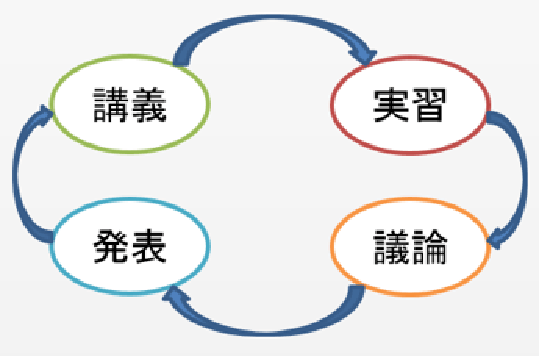
\includegraphics[height=10cm,width=13cm]{sample2.pdf}
\caption{アクティブ・ラーニングの大まかな流れ}\label{サンプル図}
\end{figure}




\section{アクティブ・ラーニングの歴史的背景}

米国では1960年代以降,高等教育が大衆化したために,従来型(講義中心)の大学教育に適応できない学生が急増した.これにより学生向けの指導方法・学習方法を研究する中で,アクティブ・ラーニングの考え方が提唱された.

アクティブ・ラーニングの解説では,ラーニング・ピラミッド(Learning Pyramid)というモデルを引用して説明されることが多い.ラーニング・ピラミッド(Learning Pyramid)のは,米国のエドガー・デール(EdgarDale)が,「学習指導における視覚的方法」の57項の中で提唱した.学習の定着率が,講義で学んだ場合は5\%,本を読んで学ぶ場合は10\%.また,人に教えた場合は90\%,といった具合に,主体的に活動するほど高まる.そして,その定着率がピラミッド状になるというモデルである.他人にものを教えることで理解が深まるといったことは,多くの人が経験しているため,ラーニング・ピラミッドは説得力があるように思われている.しかし,なぜその数値となるのか根拠になる論文は見つかっておらず不明なままである.



%図の挿入
\begin{figure}[h]
\centering
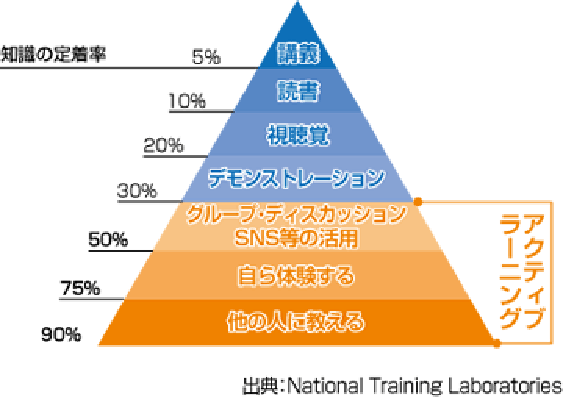
\includegraphics[height=11cm,width=13cm]{P.pdf}
\caption{ラーニング・ピラミッド}\label{サンプル図}
\end{figure}


\section{アクティブ・ラーニングの定義}
アクティブ・ラーニングの定義には様々なものがあるが,決定版となるものはまだないようである.有名なものをいくつか紹介する.

\begin{description}

 \item [中央教育審議会の定義]\mbox{}\\
 中央教育審議会は,アクティブ・ラーニングを次のように定義している\cite{中央教育審議会の定義}.

	   「教員による一方向的な講義形式の教育とは異なり,学修者の能動的な学修への参加を取り入れた教授・学習法の総称.学修者が能動的に学修することによって,認知的,倫理的,社会的能力,教養,知識,経験を含めた汎用的能力の育成を図る.発見学習,問題解決学習,体験学習,調査学習等が含まれるが,教室内でのグループ・ディスカッション,ディベート,グループ・ワーク等も有効なアクティブ・ラーニングの方法である.」

 \item [Bonwell\$Eison の定義]\mbox{}\\
Bonwell\$Eisonはアクティブ・ラーニングの一般的特徴として次のように挙げている.
 
	       \begin{itemize}
	         \item 学生は、授業を聴く以上の関わりをしていること
	         \item 情報の伝達より学生のスキルの育成に重きが置かれていること
	         \item 学生は高次の思考(分析、総合、評価)に関わっていること
	         \item 学生は活動(例:読む、議論する、書く)に関与していること
	         \item 学生が自分自身の態度や価値観を探究することに重きが置かれていること
	         \item 認知プロセスの外化を伴うこと
	        \end{itemize}

 \item [溝上慎一の定義]\mbox{}\\
  京都大学の溝上慎一教授は,アクティブ・ラーニングを次のように定義している.
 
	    「一方向的な知識伝達型講義を聴くという(受動的)学習を乗り越える意味での,あらゆる能動的な学習のこと.能動的な学習には,書く・話す・発表するなどの活動への関与と, そこで生じる認知プロセスの外化を伴う.」

\end{description}

\section{アクティブ・ラーニングへの期待}
次期学習指導要領でアクティブ・ラー二ングへの期待が高まっている.中央教育審議会(2012年8月28日)の報告書では次のように述べている.

「生涯にわたって学び続ける力,主体的に考える力を持った人材は,学生からみて受動的な教育の場では育成することができない.従来のような知識の伝達・注入を中心とした授業から,教員と学生が意思疎通を図りつつ,一緒になって切磋琢磨し,相互に刺激を与えながら知的に成長する場を創り,学生が主体的に問題を発見し解を見いだしていく能動的学修(アクティブ・ラーニング)への転換が必要である.すなわち個々の学生の認知的,倫理的,社会的能力を引き出し,それを鍛えるディスカッションやディベートといった双方向の講義,演習,実験,実習や実技等を中心とした授業への転換によって,学生の主体的な学修を促す質の高い学士課程教育を進めることが求められる.学生は主体的な学修の体験を重ねてこそ,生涯学び続ける力を修得できるのである.」


\section{大学教育におけるアクティブ・ラーニングの在り方}
中央教育審議会では,,以下のように述べている.

「大学教育の質的転換を実践していくには,学生の主体的な学修を支えるための教育方法の転換と教員の教育能力の涵養が必要である.それには,研究能力の一層の向上が求められる.双方向の授業を進め,十分な準備をしてきた学生の力を伸ばすには,教員が当該分野及び関連諸分野の学術研究の動向に精通している必要があり,教員が自らの研究力を高める努力を怠らないことが大切である.学士課程答申で指摘されているとおり,研究という営みを理解し,実践する教員が,学生の実情を踏まえつつ,研究の成果に基づき,自らの知識を統合して教育に当たることは大学教育の責務である.教育と研究との相乗効果が発揮される教育内容・方法を追求することが,一層重要である.」
また,学生の主体的な学修を促す具体的な教育の在り方は,それぞれの大学の機能や特色,学生の状況等に応じて様々である.


%図の挿入
\begin{figure}[h]
\centering
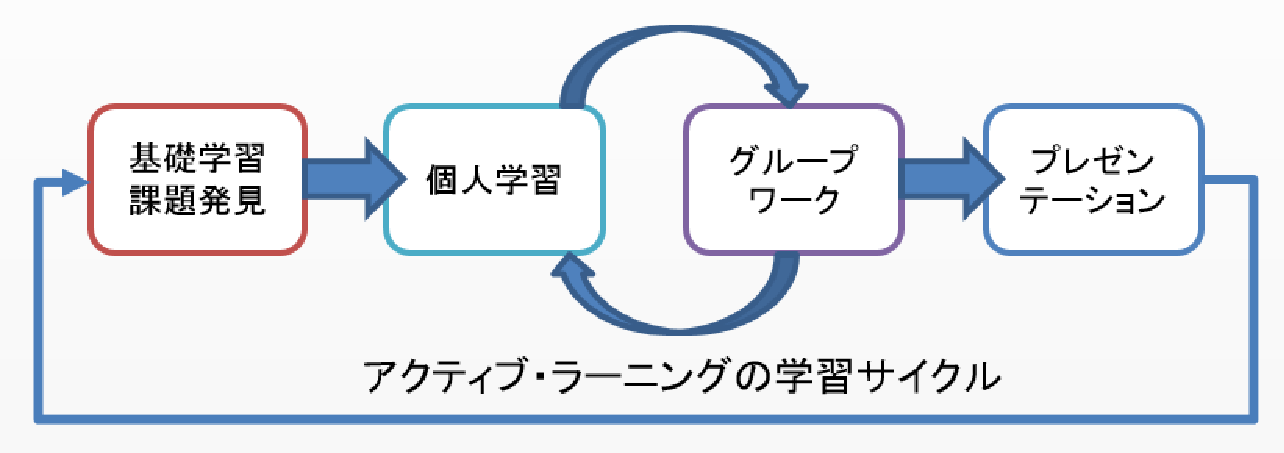
\includegraphics[height=9cm,width=13cm]{sozai3.pdf}
\caption{アクティブ・ラーニングの大まかな流れ2}\label{サンプル図}
\end{figure}

\newpage

\section{アクティブ・ラーニングを取り入れた授業の事例}

アクティブ・ラーニングには,主にTeamBasedLearning(TBL・ワークショップ型学習と呼ばれる(WorkshopBasedLearning)略してWBL)・課題解決学習(ProblemBased,略してPBL)という3つの教育方法がある.後者になればなるほど,学生の主体的な取り組み具合が高くなる.いずれも専用の授業時間で行われるが,常時実施できないため,これらの授業だけでは学生に主体的な学習を定着させることが難しい.そこでいくつかアクティブ・ラーニングを導入した授業についていくつか事例を紹介する\cite{事例}.\\

女子栄養大学短期大学部の成功事例\vspace{0.2in} \\*
先生ごっこ\\
授業中に行われる「先生ごっこ」とは,学生が2~3人のグループをつくり,10分程度の間に先生によって説明されたイラストを交代で相手に教え合う.この手法はピア・インストラクション(PeerInstruction)といい,学生同士の議論を組み込んだアクティブラーニング型授業の一つである.ConcepTest(概念を測定する質問)と呼ばれる課題を出し,クリッカーなどを使って個々の学生の理解度をはかるとともに,学生同士の議論を通じて深い理解を促す効果がある.協同学習やPBL(Project-Based Learning)のような演習的な授業ではなく,基本的な知識を扱う講義型授業で行われること,授業外学習とリンクさせていることも,ピア・インストラクションの特徴である.

そして「人に教える」という行為がもっとも学習を促進するといわれるが,この授業にはまさにこれが実現されている.高学力の学生にとっては,将来栄養士として一般の方に「教える」という訓練となり,低学力の学生は相手から教わり,自ら教えるという努力を通して理解を進めることができる.また,小さな成功体験を積み重ねることが,モチベーションを高める駆動力にもなっている.「先生ごっこ」のひとときは,学生同士が教え合うとりわけ活気ある光景が教室に展開されている.この「先生ごっこ」において留意されているのは,教えあうべき内容の指示がかなり明確である点である.この講義では,「今,教授が説明した1枚のイラストを学生が説明する」という指示であるため学生は「何をしてよいかわからない」状態に陥ることがない.また、互いに教え合った後は,先生役の説明の出来映えについて簡単な評価シートに書き込まれる.「聞く・話す・書く」がバランスよく構成され,授業がテンポよく進行するため,学生が飽きる・寝るということがなくクラス全体の雰囲気が終始活気に満ちている.

また,この授業では反復学習といい,一つのトピックの学習が何度も反復されるよう設計されている.予習段階で課題に取り組み予習内容についての確認テストを行うため,学生は少なくとも2回トピックにふれる.授業中には教員からの説明,先生ごっこ(生徒役),先生ごっこ(先生役)において3回トピックにふれる.そして,翌週にミニ確認テストとして,期末テスト時にも1回ふれる.さらには,前期の講義内容を数ヶ月経過後の後期の授業中に復習テストとして行う.これらを合計すると少なくとも8回はそのトピックにふれる機会がある.これだけの反復が設計されており、学習内容の定着率をかなり上昇させる構造となっている.

このピア・インストラクションの手法を用いた授業では,学生は小さな成功を多く経験し,そのことが自信とさらなる勉強に対する動機づけとなっている.この作用は,基礎学力の低い学生に,高い学生より有意に多くみられ効果の高いことを示している.\vspace{0.3in} \\*

金城学院大学\vspace{0.2in} \\*
組織的・重層的なPBL\\
初めに1年生を12~13人ずつのグループに分け,学科の教員が持ちまわりで各グループに毎回1名つく.さらに,その教員の「薬学セミナー」生である2年生4~5名がチューターとして参加する.1つの課題は2週間(1コマ90分×4回+授業外学習)で完結するというものである.1年生12~13人は課題ごとに1つの司会グループと調査・発表グループの2グループに分かれる.教員およびそのセミナー生は課題ごとに変わるが,1年生12~13人ずつのグループは固定で,1年間に4回ほど組み替えがある.2年生が正課授業の一環として1年生のサポートにまわることで,2年生が1年生にとっての格好のロールモデルになり,2年生にとっても貴重な学習機会でもある.

2週間の授業の流れは,1回目の授業では,司会グループの1年生が2年生の協力を得ながら司会を担当する.興味あるテーマについて意見交換をしながら,テーマと調査内容・方法を決める.この過程で疑問点を明らかにし,調査内容を熟考を重ねる.更に,調査事項をグループで文献やインターネットを使って調査する.2回目の授業で1年生全員がPC教室に集まり,PCや書籍を使って調査,レジュメ作成を行う.3回目の授業では,2つの調査・発表グループが発表し,質疑応答を行う.発表後,チューターおよび教員からアドバイスを受ける.その後,発表および司会に関する評価シートと振り返りを提出する.4回目の授業では,1年生全員がPC教室に集まり,各々の司会グループがグループ内発表の内容を報告する.そして教員が総括し,振り返りシートを記入するという流れである.持ちまわりの教員およチューターの2年生は,1回目と3回目の授業に参加し,チューターの2年生は必要に応じて1年生に適切なアドバイスをおくり,サポートすると共に,教員による1年生の評価にも参加する.これは人を客観的に見て評価する訓練に役立てるとともに,複数の目で1年生の学習態度やレジュメをチェックすることにより,学習評価の妥当性や信頼性を向上させることに繋がる.

このグループディベート型討議方式を授業に取り入れることで,サブグループ間の仲間意識を刺激し,コミュニケーション能力が向上するという効果が表れた.また,能動的に学ぶ態度を養成できるという効果も得た事例である.



%図の挿入
\begin{figure}[h]
\centering
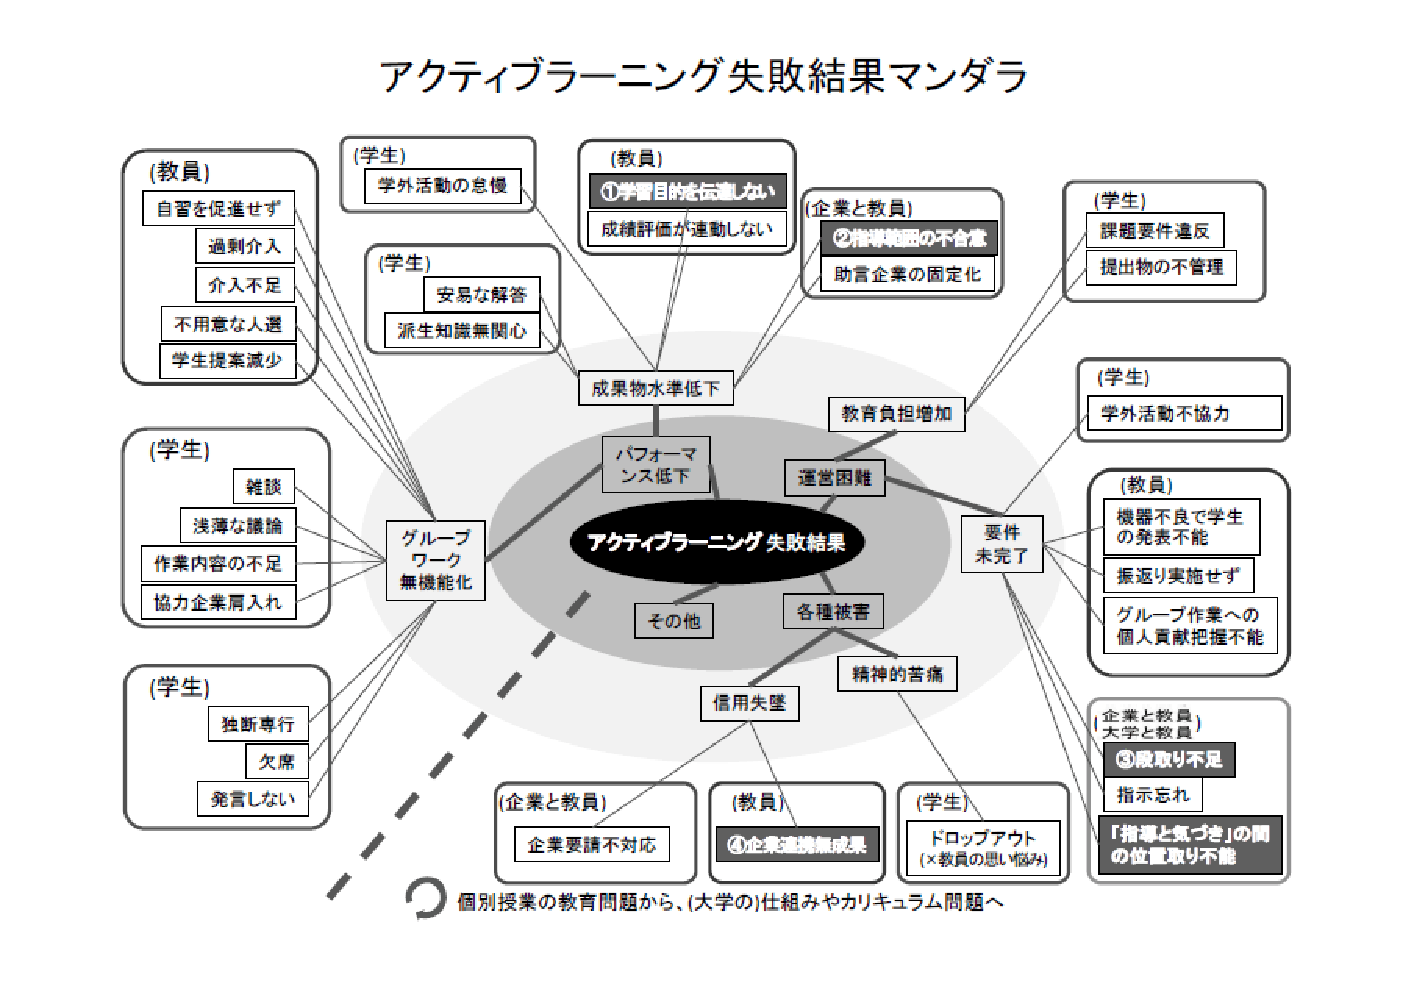
\includegraphics[height=11cm,width=13cm]{kekka.pdf}
\caption{アクティブ・ラーニング失敗結果マンダラ}\label{サンプル図}
\end{figure}


%図の挿入
\begin{figure}[h]
\centering
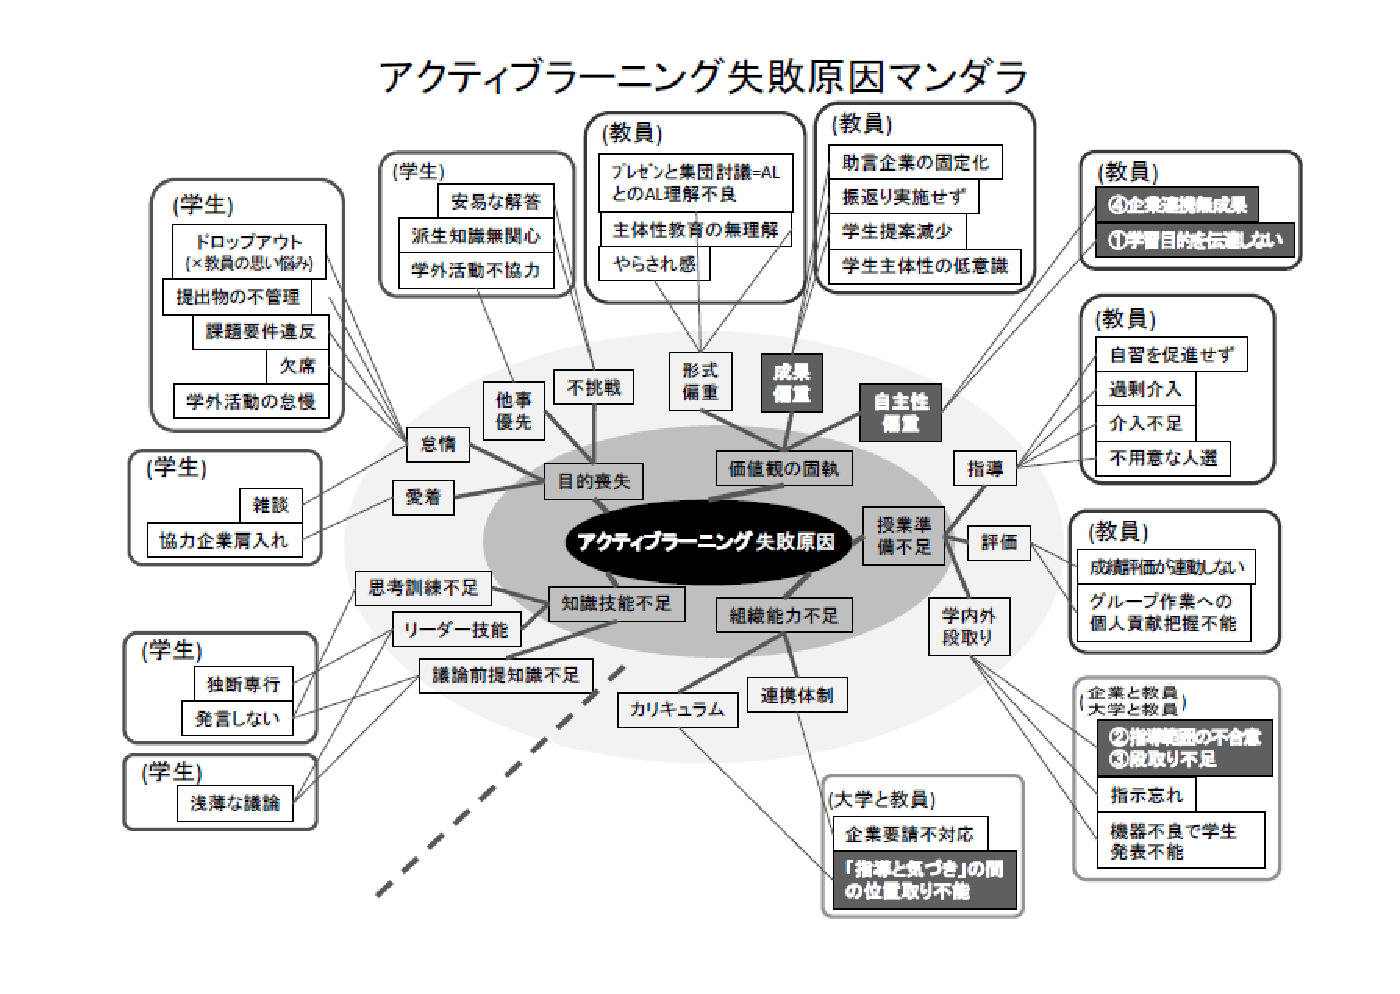
\includegraphics[height=11cm,width=13cm]{geiin.pdf}
\caption{アクティブ・ラーニング失敗原因マンダラ}\label{サンプル図}
\end{figure}





\chapter{日本の教育政策の現状について}

\section{学習指導要領とは}

学習指導要領は,教育基本法に定められた教育の目的などの実現を図るため,学校教育法に基づき国が定める教育課程の基準であり,教育の目標や指導すべき内容などを示す\cite{学習指導要領}.各学校は,学習指導要領に基づき,その記述のより具体的な意味などについて説明した教科など別の解説も踏まえつつ,地域の実状などに即して教育課程が編成され,年間指導計画や授業ごとの学習指導案等が作成・実施されている.

これまで学習指導要領は,時代の変化や子供たちの状況,社会の要請などを踏まえ,約10年ごとにわたり改訂されてきた.例えば,我が国が工業化という共通の社会的目標に向けて,教育を含めた様々な社会システムを構想し構築していくことが求められ,昭和33年の改訂した.また,高度経済成長が終わりを迎える中で個性重視のもと「新しい学力観」を打ち出した平成元年の改訂など,時代や社会の変化とともに,学習指導要領の改訂も重ねられてきた.

時代の変化や社会の要請など,その時点での成果と課題の検証を踏まえながら,未来に向けてふさわしい学校教育の在り方を構築するという作業の積み重ねの上に,学習指導要領は築かれてきた.


%図の挿入
\begin{figure}[hp]
\centering
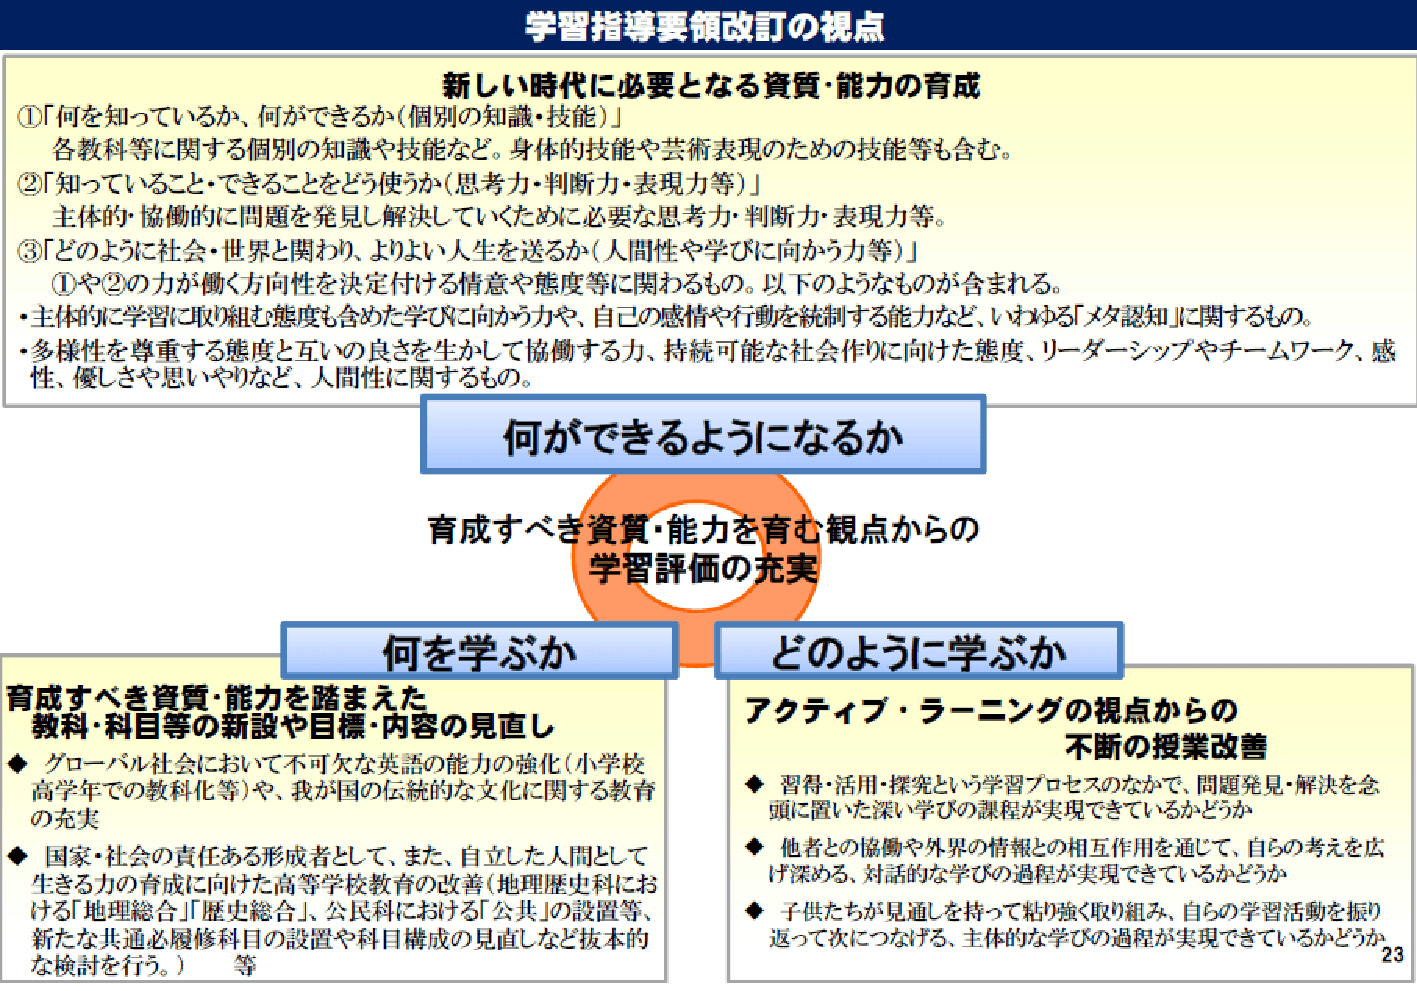
\includegraphics[height=13cm,width=13cm]{gakusyuu.pdf}
\caption{学習指導要領改訂の視点}\label{サンプル図}
\end{figure}


\section{幼児教育}
資質・能力の三つの柱を踏まえ,幼児教育で育みたい資質・能力として,「知識・技能の基礎」,「思考力・判断力・表現力等の基礎」、「学びに向かう力,人間性等」の三つを重視するようになり,自己制御や自尊心などのいわゆる非認知的能力の育成など,現代的な課題を踏まえた教育内容の見直しを図るとともに,預かり保育や子育ての支援も充実するようになった.5歳児修了時までに育ってほしい具体的な姿を明確にし,幼児教育の学びの成果が小学校と共有されるよう工夫・改善された.また,幼稚園教育要領の改訂内容と保育所保育指針及び幼保連携型認定こども園教育・保育要領の改訂内容との整合性を図り,幼児教育全体としての質を確保・向上されることとなった.

\section{初等中等教育}

小学校の6年間は,子供たちにとって大きな幅のある期間である.低学年,中学年,高学年の発達の段階に応じた資質・能力の在り方や指導上の配慮が必要になる.小学校の学びはゼロからスタートするのではなく,幼児期の学びの上に育まれるものであり,生活科を中心とした「スタート・カリキュラム」などを通じて,保幼小連携を図っていくことが重要である.また,小・中学校間で育成すべき資質・能力を共有し,義務教育9年間を通じた資質・能力の育成を図ることが重要であり,学習や生活の基盤作りという観点から,初等教育の段階における言語能力の育成は極めて重視されている.

国語教育においては,小学校低学年で表れた学力差が,その後の学力差の拡大に大きく影響するとの指摘があり,学習の質に大きく関わる語彙量を増やし語彙力を伸ばすための指導や,文や文章の構成を理解したり,複数の情報を関連付けて理解を深めたりするための指導が充実されるよう,育成すべき資質・能力を明確化し,それを育む指導内容に移行された.外国語教育については,外国語で多様な人々とコミュニケーションを図ることができる基礎的な力を育成することが重要であり,小・中・高等学校を通じて一貫して育む指標形式の目標を設定し,初等中等教育全体を見通して確実に育成された.

文部科学大臣は,平成26年11月20日に中央教育審議会に対して,次期学習指導要領に関して検討を行うように諮問した.諮問文「初等中等教育における教育課程の基準等の在り方について(諮問)」では,次のようにいう\cite{初等中等教育における教育課程の基準等の在り方について}.

「必要な力を子供たちに育むためには,「何を教えるか」という知識の質や量の改善はもちろんのこと,「どのように学ぶか」という,学びの質や深まりを重視することが必要であり,課題の発見と解決に向けて主体的・協働的に学ぶ学習(いわゆる「アクティブ・ラーニング」)や,そのための指導の方法等を充実させていく必要があります.こうした学習・指導方法は,知識・技能を定着させる上でも,また,子供たちの学習意欲を高める上でも効果的であることが,これまでの実践の成果から指摘されています.」

従来は大学教育で用いられてきた「アクティブ・ラーニング」が初等中等教育でも中心的課題として取り上げられた.また,中央教育審議会が平成26年12月22日に発表した「新しい時代にふさわしい高大接続の実現に向けた高等学校教育,大学教育,大学入学者選抜の一体的改革について〜すべての若者が夢や目標を芽吹かせ,未来に花開かせるために〜(答申)」においても,高校教育及び大学教育の両方において,「アクティブ・ラーニング」を積極的に導入していくことが記されている.

\newpage

\section{高等教育}

大学審議会の「グローバル化時代に求められる高等教育の在り方について(答申)」では,次のようにいう\cite{グローバル化時代に求められる高等教育の在り方について}.

「社会,経済,文化のグローバル化が急速に進展し,国際的な流動性が高まっている.科学技術の爆発的な進歩と社会の高度化,複雑化や急速な変化に伴い,過去に蓄積された知識や技術のみでは対処できない新たな諸課題が生じており,これに対応していくため,新たな知識や専門的能力を持った人材が求められている.平成11年6月のケルンサミットでは,生涯にわたる学習機会の確保と、学生、教員等の国際交流の重要性が強調され,教育の在り方を見直す必要性については,日本にのみに限らず国際的にも共通の認識となった.このような中で,大学などの高等教育機関は,知的資源を世界に向けて発信し,世界の人々に対して高度な知識や技術を伝えることにより,世界に開かれた高等教育機関としての役割をなお一層果たすことが期待されている.」

平成10年10月の答申「21世紀の大学像と今後の改革方策について」では,21世紀初頭の社会状況を展望し,日本の高等教育が世界的水準の教育研究を展開し,期待される役割を果たしていくために,改革に向けた四つの基本理念「1.課題探求能力の育成を目指した教育研究の質の向上,2.教育研究システムの柔構造化による大学の自律性の確保,3.責任ある意思決定と実行を目指した組織運営体制の整備,4.大学の取組についての多元的な評価システムの確立による大学の個性化と教育研究の不断の改善」という改革方策を示した.

一方,中央教育審議会答申「初等中等教育と高等教育との接続の改善について」(平成11年12月)においては,大学教育における今後の課題として,国際化や生涯学習社会の一層の進展に対応した大学の在り方についての検討が求められている. 今後,高等教育制度の国際的な整合性を図り,教育研究のグローバル化を推進するとともに国際競争力を高めることが重要である.これを通じて質の高い高等教育を提供し,世界のあらゆる分野で活躍し得る能力を持った人材の育成に貢献していくことが求められることになったのである.

\newpage

\section{大学教育}
グローバル化や少子高齢化,情報化といった急激な変化の中,雇用構造や労働市場の変化も加わった先の見え難い時代を生きる若者や学生にとって,「生涯学び続け,どんな環境でも勝負できる能力」の育成や知的な基礎に裏付けられた技術や技能などの習得は切実な問題である.今後の変化に対応するための基礎体力を固め直し,先端的な活路を見出したりする原動力となる人材を切望している.

中央教育審議会が平成24年8月28日に発表した「新たな未来を築くための大学教育の質的転換に向けて〜生涯学び続け,主体的に考える力を育成する大学へ〜(答申)」では次のように述べる\cite{中央教育審議会の定義}.

「高校までの勉強から大学教育の本質である主体的な学修へと知的に跳躍すべく,学生同士が切磋琢磨し,刺激を受け合いながら知的に成長することができるよう,課題解決型の能動的学修(アクティブ・ラーニング)といった学生の思考や表現を引き出しその知性を鍛える双方向の授業を中心とした質の高いものへと学士課程教育の質を転換する必要がある.」


%図の挿入
\begin{figure}[h]
\centering
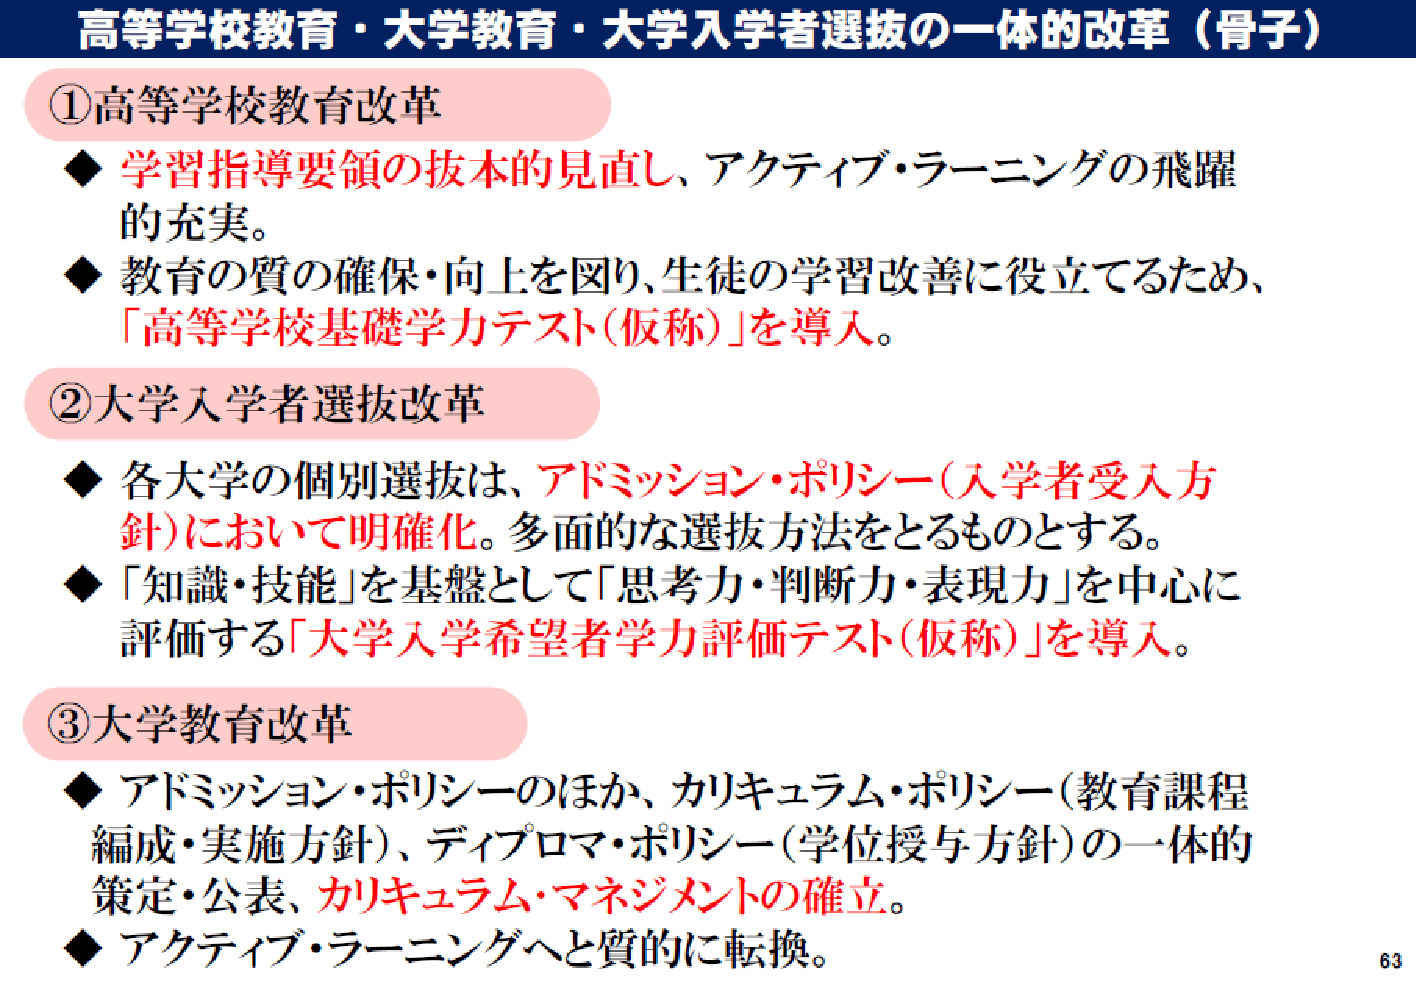
\includegraphics[height=13cm,width=13cm]{daigaku.pdf}
\caption{高等学校教育・大学教育の改革}\label{サンプル図}
\end{figure}

\newpage

\section{子供たちの現状と課題}

学習指導要領の改訂に当たって議論の論点となるのは,子供たちの現状や課題についての分析と、今後活躍するであろう子供たちの将来についての見通しである.
学力については,国内外の学力調査の結果によると近年改善傾向にあり,子供たちの学習時間は増加傾向にあるという調査結果もある.また,選挙権年齢が引き下げられてから初の選挙となった第24回参議院議員通常選挙における18歳の投票率は若年層の中では高い割合となり、選挙を通じて社会づくりに関わっていくことへの関心の高さをうかがわせた.こうした調査結果から,学習への取組や人とのつながり,地域・社会との関わりを意識し,関わっていこうとすることがわかる.
こうした中で,内閣府の学力に関する調査においては,判断の根拠や理由を明確に示しながら自分の考えを述べたり,実験結果を分析して解釈・考察し説明したりすることなどについて課題が指摘されている.調査結果から,自らの能力を引き出し,学習したことを活用して,生活や社会の中で出会う課題の解決に主体的に生かしていくという面からみた学力は,課題があることがわかる.

また,スマートフォンなどの普及に伴い,情報技術(ICT)を利用する時間は増加傾向にある.その一方で,子供たちが読書をしなくなる傾向にあり,教科書の文章を読み解けていないとの調査結果がある.情報化が進展しあらゆる分野の多様な情報に触れることがますます容易になる一方で,視覚的な情報と言葉との結びつきが希薄になり,知覚した情報の意味を吟味して読み解くことが少なくなっているのではないかと考えられる.文章で表された情報を的確に理解し,自分の考えの形成に生かしていけるようにすることは緊要の課題である.特に,小学校低学年における学力差はその後の学力差に大きく影響すると言われており,語彙の量と質の違いが学力差に大きく影響しているとの指摘もあり,言語能力の育成は前回学習指導要領の改訂に引き続き課題となっている.







\chapter{目的}

\section{研究目的}
本研究では,学習者自身を被験者とする.PM学科のPMコース・JABEEコースのデータマイニング入門を受講した学生を対象に,アクティブ・ラーニングをデータマイニング教育に取り入れ,受講者の能動的な学習への参加を取り入れた能力の育成を図る.受講者自身は,与えられたデータをマイニングするだけではなく,データをどうやって集めるか,データ収集法の設計から考え,学習する.最終的には今回の実践結果をフィードバックし,今後の教育に役立ててもらうことを目指す\cite{アクティブ・ラーニング1}.

\chapter{手法}

\section{研究手法}

この計画は4週間に分けて行う.対象は千葉工業大学データマイニング入門を受講している学生とする.
初めに,各グループ4,5人になるようランダムに振り分ける.
次に勉学に関する質問を題材とし,データを収集する.そこで何を知りたいか考え,またどのようにしてデータ収集するか,各グループ3つずつ質問を考えてもらう.各グループが考えた質問をGoogleフォームにまとめ,アンケートを作製し,すべての学生に回答してもらう.解析手法を学んだ後,自分のグループの質問結果と全ての質問結果の2つをデータマイニングしてもらい,その結果からわかったことを発表してもらう.

\chapter{データマイニング入門ついて}

\section{データマイニングとは}

データマイニングとは,1990 年代中頃から用いられるようになった言語であり,情報システムに蓄積した巨大なデータの集合をコンピュータによって統計学,パターン認識,人工知能などのデータ解析の技法を用いて,大量のデータの中から知識を取り出す技術のことである.テキストを対象とするものをテキストマイニング,中でもウェブページを対象にしているものはウェブマイニングと呼ばれている.データマイニングの適用分野や目的,対象となるデータの種類は多種多様であり,ビジネスの分野では企業が業務に関連して記録したデータ(過去の取引記録、行動履歴など)を元に,意思決定や計画立案,販売促進などに有効な知見を得るために行われることが多い.


\section{データマイニングの事例}
データマイニングの成功事例は,数多く報告されており,有名な話としておむつとビールの話しがある.データマイニングにバスケット分析という,POS データなどの取引データを分析する手法があり,「おむつを買った人はビールを買う傾向がある」という分析結果が1990 代半ばから2000 年台初めにかけてメディアや講演などでよく語られ,データマイニングという言葉と概念を有名にした.これは「米国の大手スーパーマーケット・チェーンで販売データを分析した結果,顧客はおむつとビールを一緒に買う傾向があることが分かった.調査の結果,子供のいる家庭では母親はかさばる紙おむつを買うように父親に頼み,店に来た父親はついでに缶ビールを購入していた.そこでこの2つを並べて陳列したところ,売り上げが上昇した」という内容である.明確な答えはないが,おむつとビールの売り場を近くにおいたことで店の売上向上につながった話もあり,データマイニングの結果から推測することで顧客の潜在的なニーズを引き出すことができる.

\newpage

\section{データマイニングのツール}

データマイニングのツールではSAS,SPSS,S言語,VisualMiningStudioなど様々なツールがある.しかしデータマイニング機能を揃えたSAS,SPSS,S言語,VisualMiningStudioなどのパッケージは値段が高価なため個人ユーザが簡単に使えるものではない.そこでデータマイニング入門の講義内では,受講者にS言語並みの機能を持つフリーソフトのRをツールとして使用してもらうこととする.

\section{アクティブ・ラーニング手法の導入・実践スケジュール}

以下に,データマイニング入門における今後のアクティブ・ラーニング手法の導入・実践スケジュールを記す.
\begin{table}[h]
  \begin{center}
    \caption{アクティブ・ラーニング手法の導入・実践スケジュール}
    \begin{tabular}{|l|l|} \hline
      日程 & 内容  \\ \hline
      10/24 & 受講者を各グループ4,5人になるよう分ける  \\
      10/31 & 各グループで勉学に関する質問を3つ考えてもらう  \\
      11/7 & Googleフォームにて質問をまとめアンケートを作成し,受講者全員に回答してもらう  \\
      12/12 & 受講者は自分のグループの質問結果と全ての質問の結果をマイニングし,発表してもらう  \\ \hline
    \end{tabular}
  \end{center}
\end{table}



\section{データマイニング入門のシラバス}
2016年度データマイニング入門のシラバスは以下の通りである.

%図の挿入
\begin{figure}[htb]
\centering
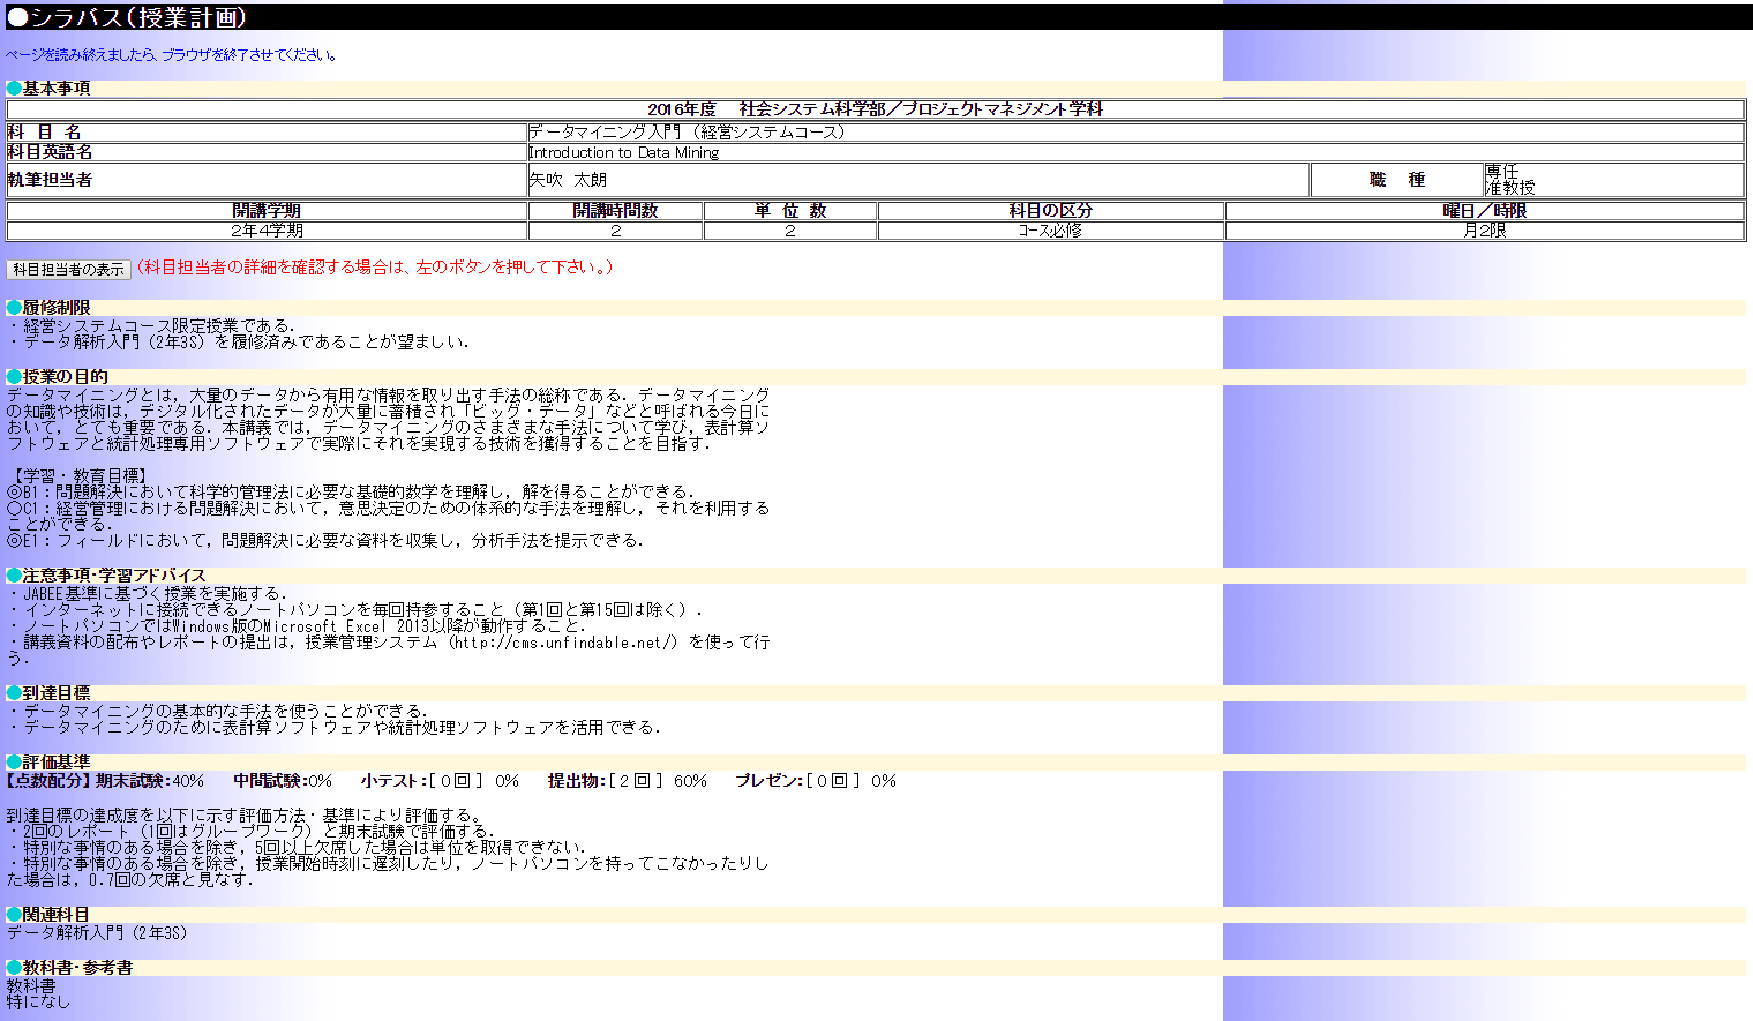
\includegraphics[height=14cm,width=13cm]{sirabasu1.pdf}
\caption{データマイニング入門シラバス1}\label{サンプル図}
\end{figure}

%図の挿入
\begin{figure}[htb]
\centering
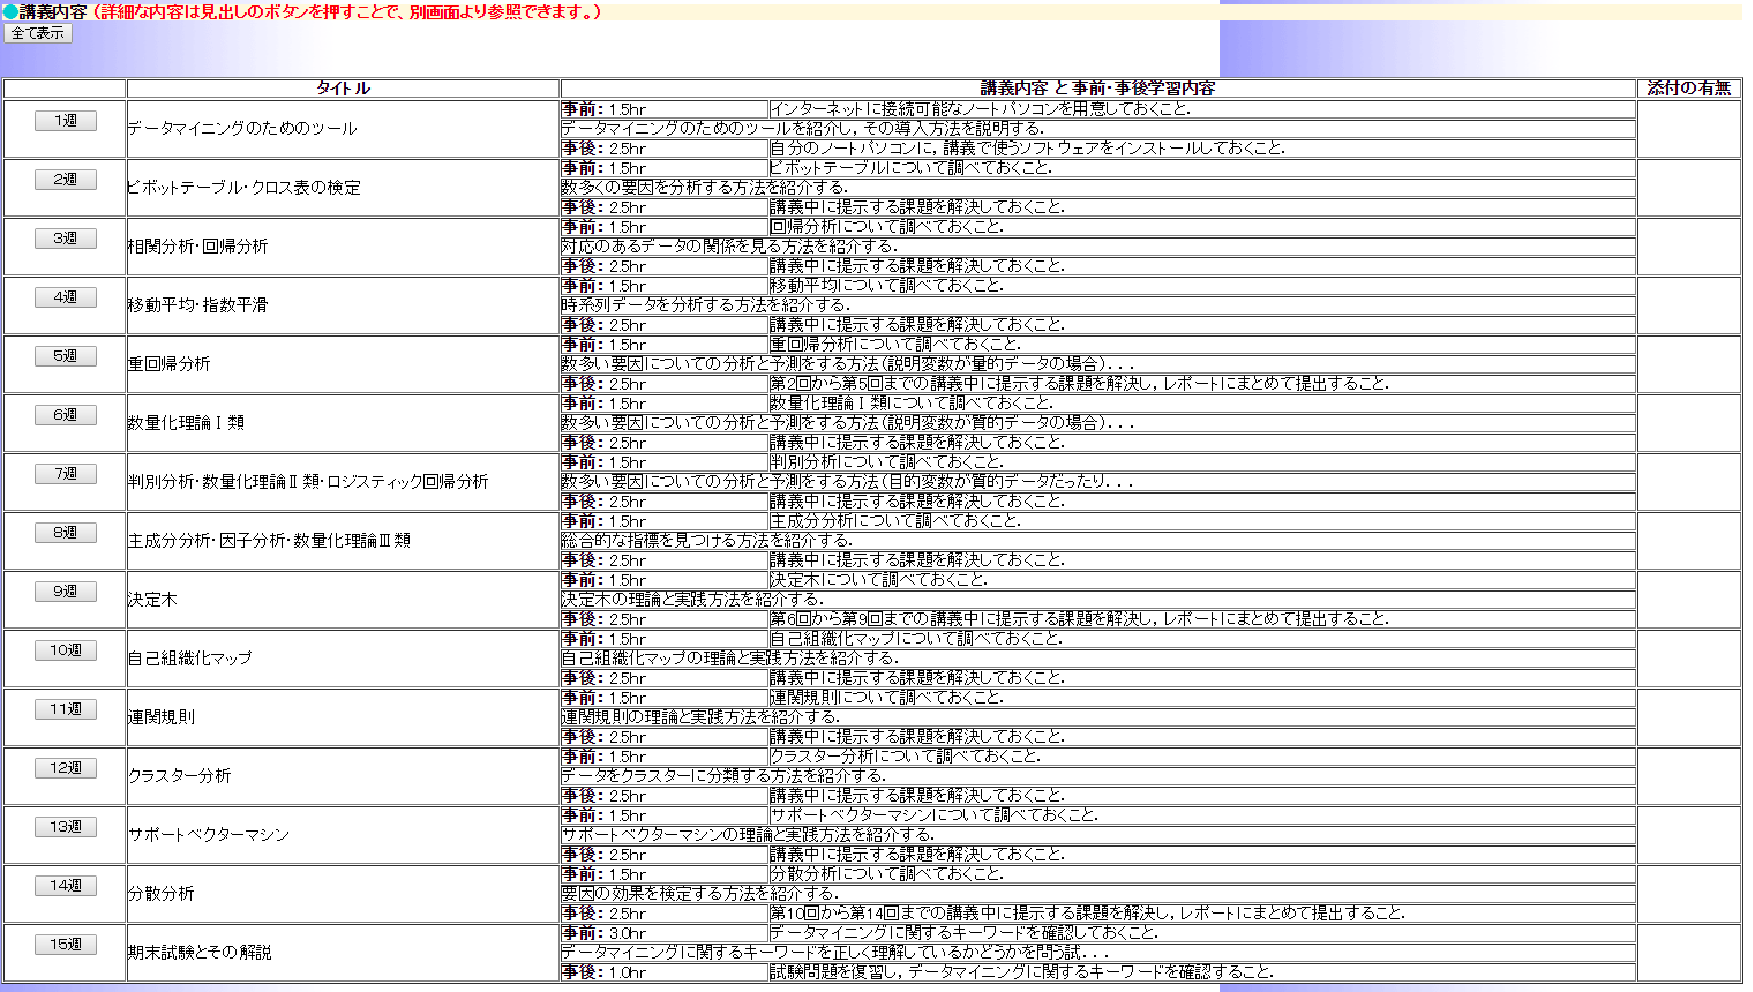
\includegraphics[height=14cm,width=13cm]{sirabasu.pdf}
\caption{データマイニング入門シラバス2}\label{サンプル図}
\end{figure}

\chapter{R言語について}

\section{R言語とは}
R言語は,ニュージーランドの統計学科のオークランド大学のRoss Ihakaと,アメリカのハーバード大学生物統計学のRobert Clifford Gentle-manにより作られた.Rの言語の名前の由来は統計解析言語であるS言語の独自実装であるので,S言語の「一歩手前」の「R」という意味や,創設者二人の頭文字であるRに由来しているという説がある.R言語は,データ分析やデータ処理に特化したオープンソースのプログラミング言語であり,システム開発をするほかのプログラミング言語とは位置づけが異なり,統計解析機能が付いていて,分析処理や,その結果をグラフィカルに表示することができる.



\section{Rの導入}
R言語はUNIX,Windows,Macなど様々なOSで使用可能である.今回は,Windows版の導入方法を記述する.

\begin{enumerate}

\item R言語のサイト(https://www.r-project.org/)にアクセスし,左上のDownloadの項目にあるCRANをクリックする.
\item 「JAPAN」の項目を探し,統計数理研究所,又は山形大学のRのミラーサイトをクリックする.
\item 画面上部にある「Download R for Windows」をクリックする.
\item 画面上部にある「base」をクリックする.
\item 「Download R 3.2.2 for Windows」をクリックするとDownloadが開始する.



\end{enumerate}

%図の挿入
\begin{figure}[p]
\centering
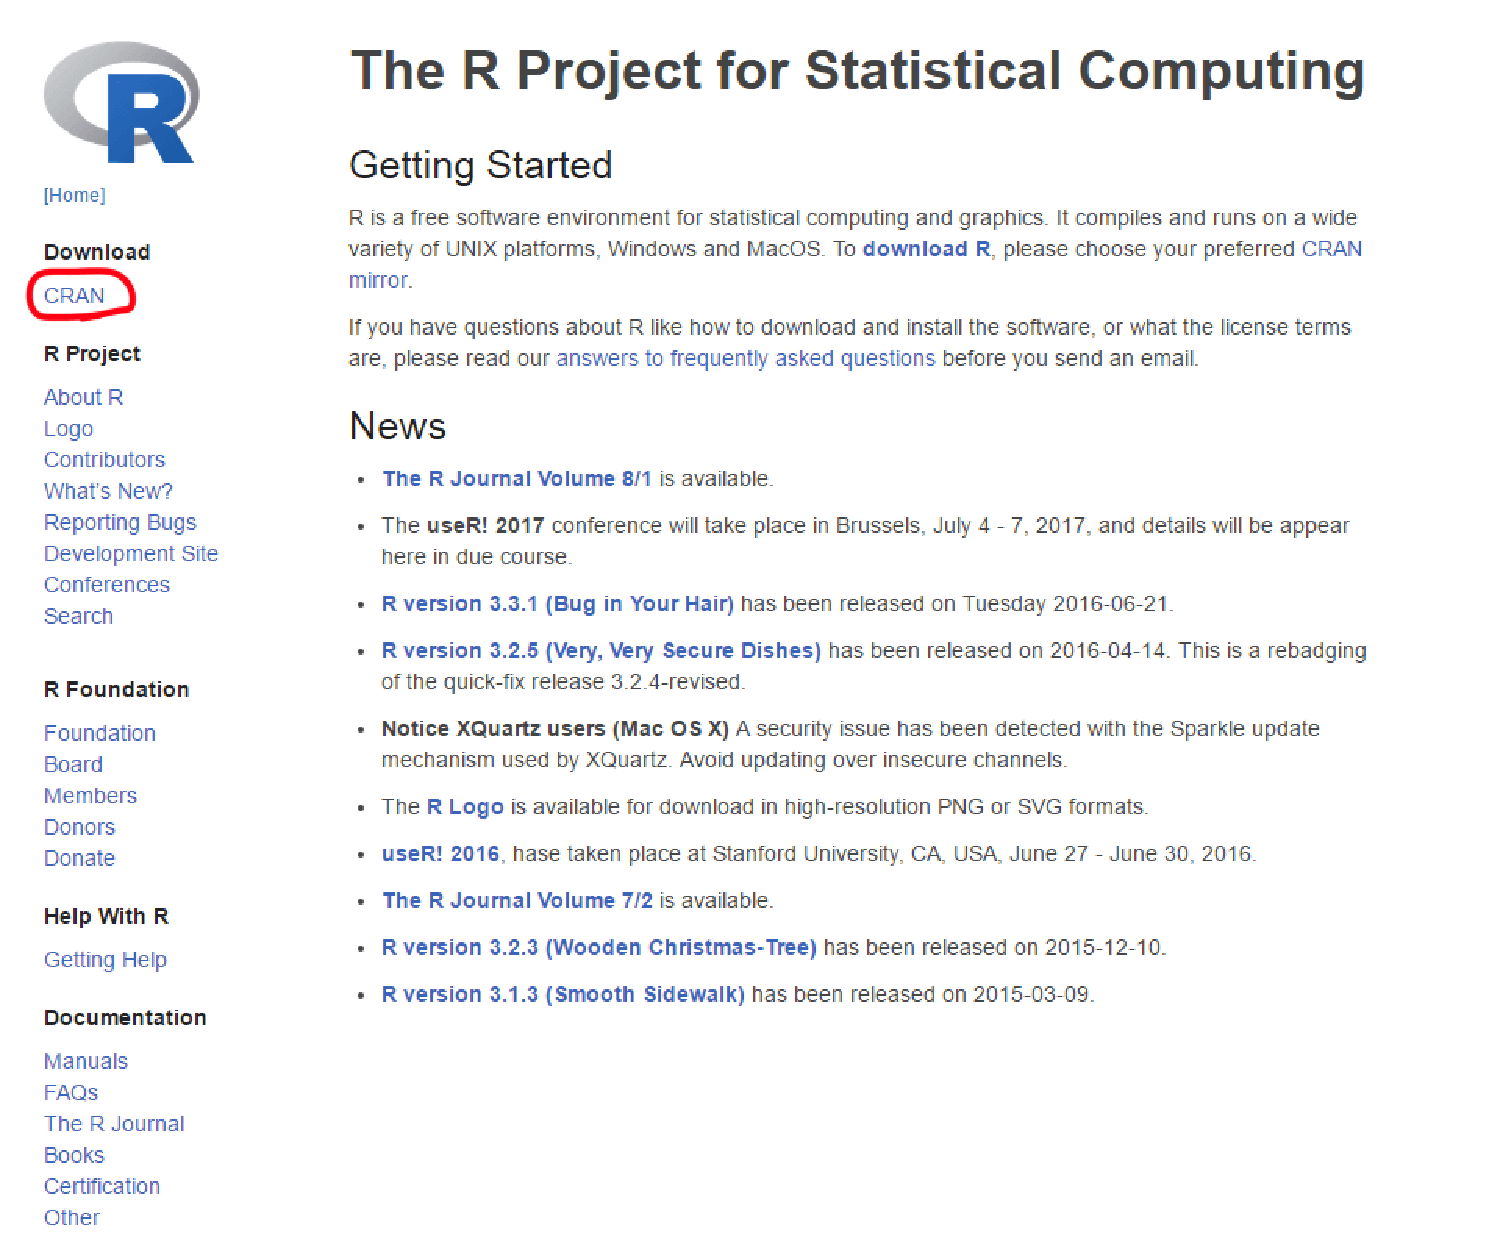
\includegraphics[width=13cm]{R1.pdf}
\caption{Rインストール手順}\label{サンプル図}
\end{figure}

%図の挿入
\begin{figure}[p]
\centering
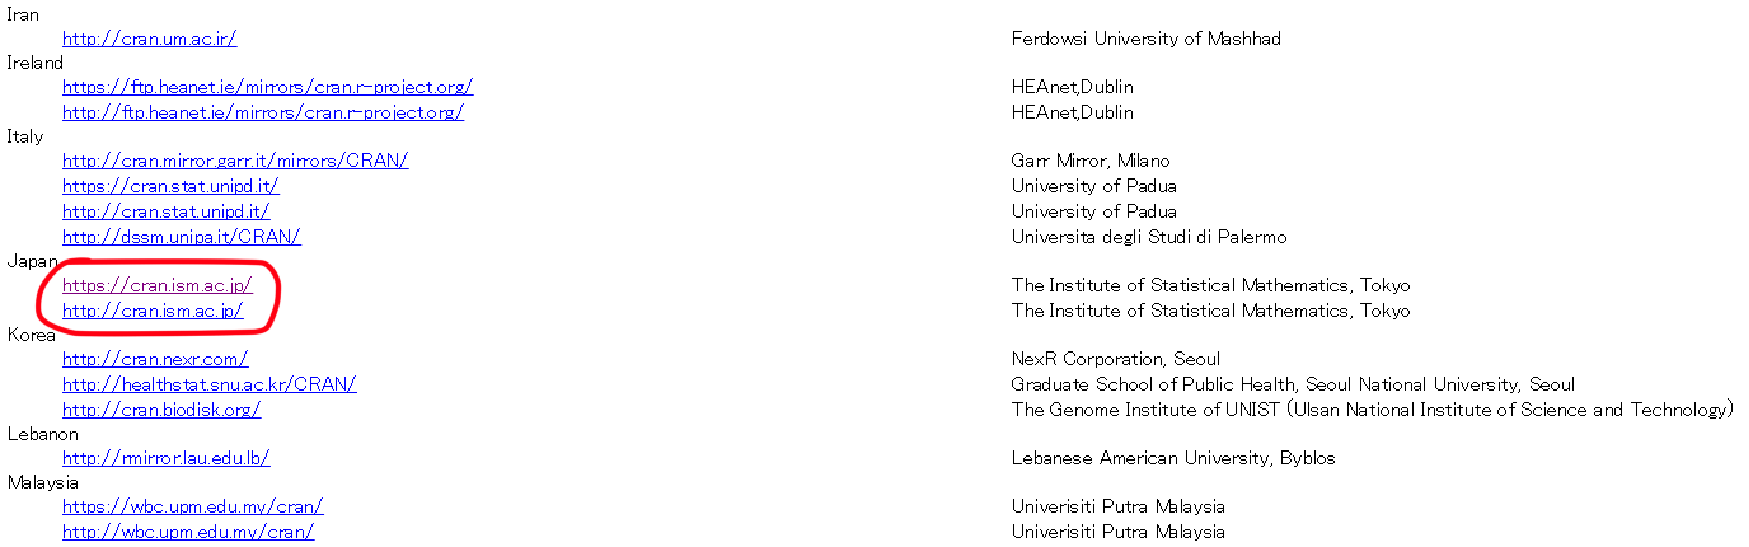
\includegraphics[width=13cm]{R2.pdf}
\caption{Rインストール手順2}\label{サンプル図}
\end{figure}

%図の挿入
\begin{figure}[p]
\centering
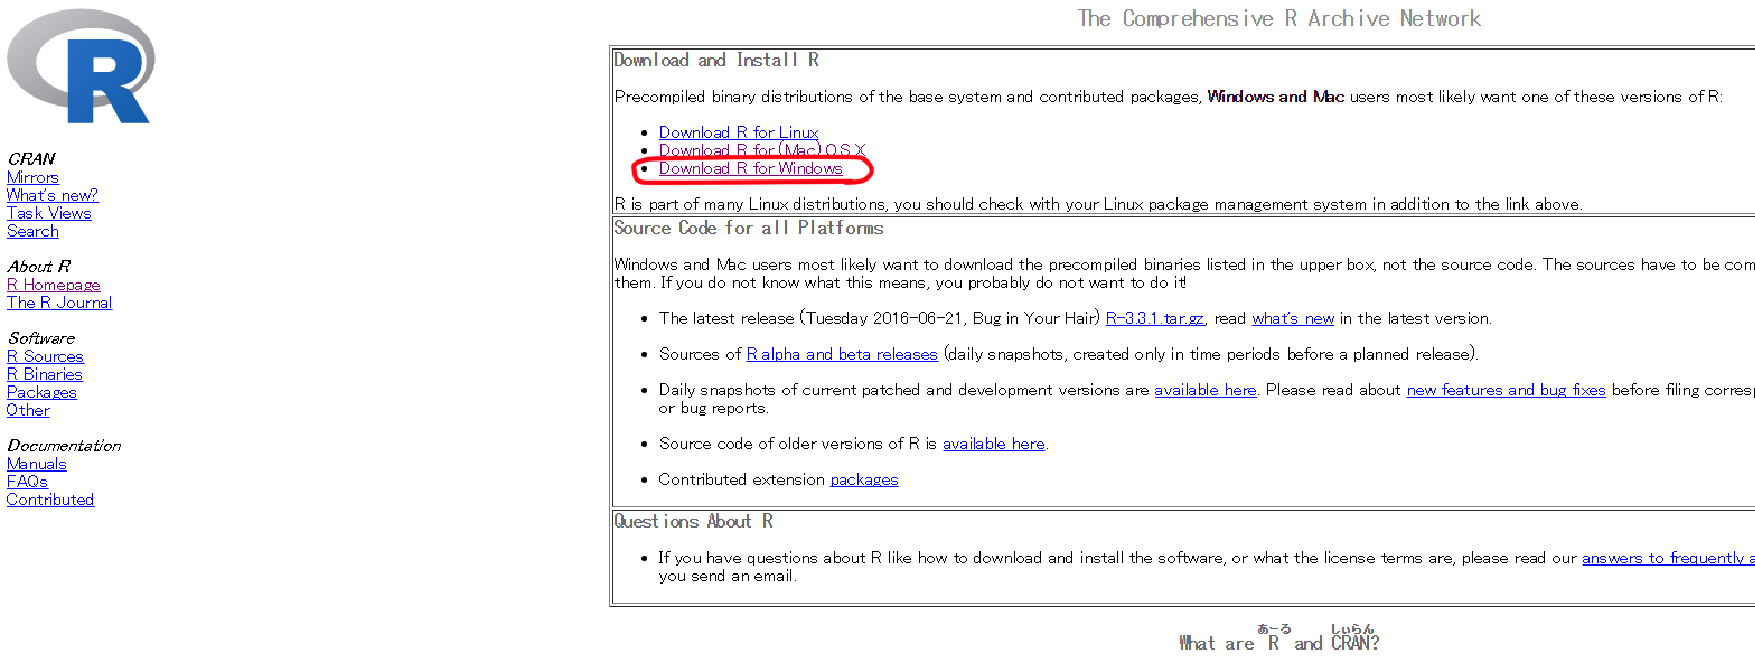
\includegraphics[height=7cm,width=13cm]{R21.pdf}
\caption{Rインストール手順3}\label{サンプル図}
\end{figure}



%図の挿入
\begin{figure}[p]
\centering
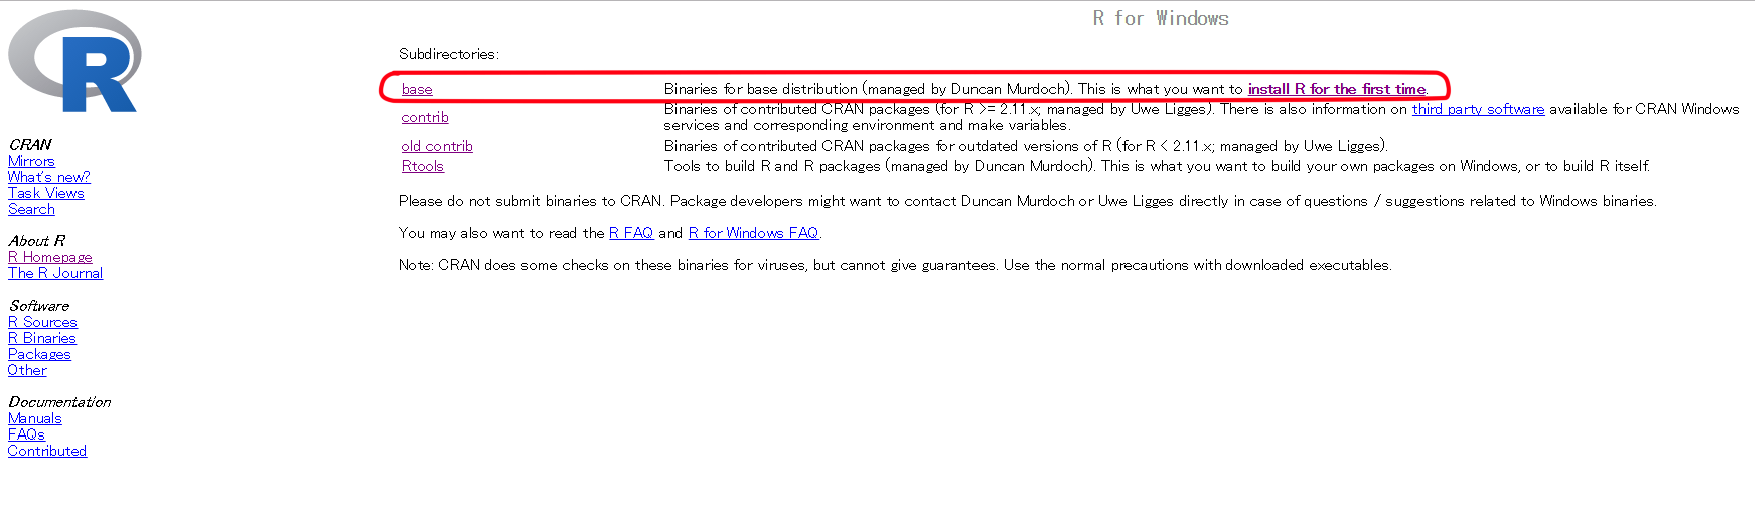
\includegraphics[height=7cm,width=13cm]{R25.pdf}
\caption{Rインストール手順4}\label{サンプル図}
\end{figure}



%図の挿入
\begin{figure}[p]
\centering
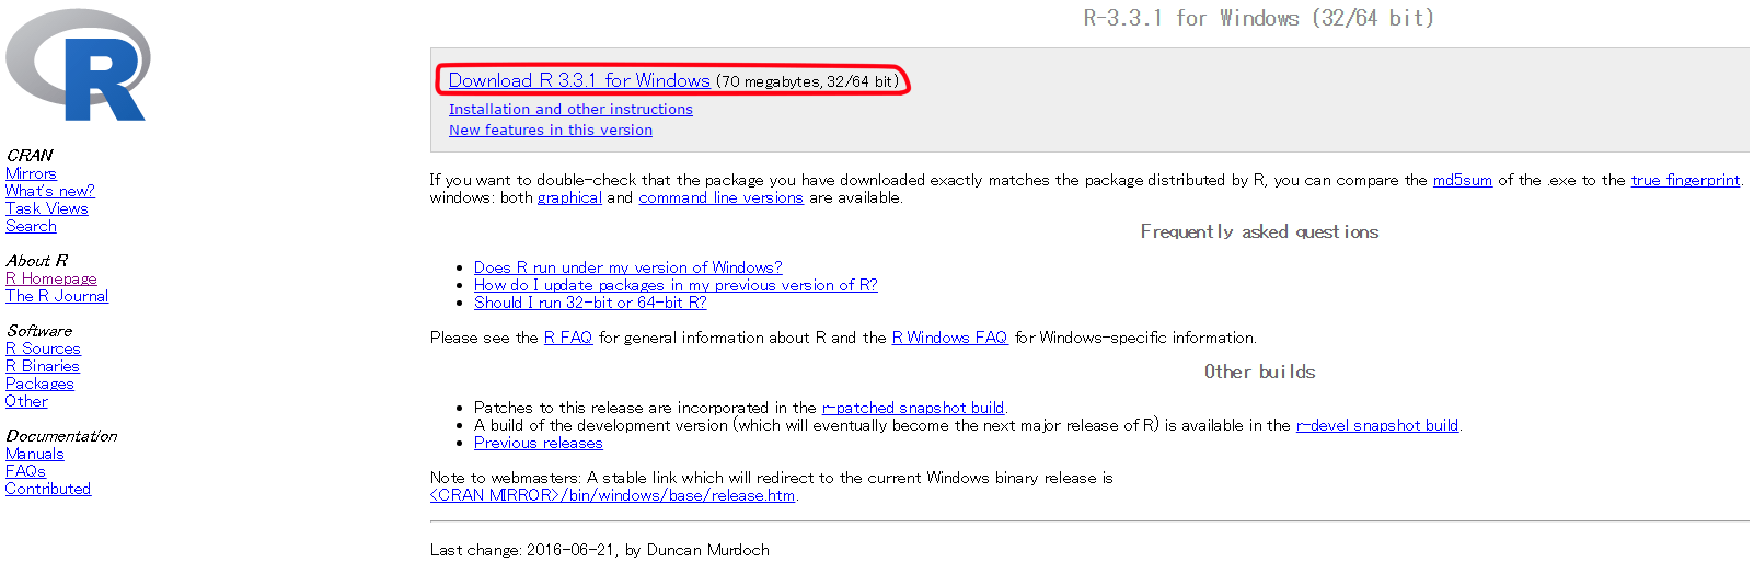
\includegraphics[height=7cm,width=13cm]{R3.pdf}
\caption{Rインストール手順5}\label{サンプル図}
\end{figure}


\newpage

\section{Rの起動と終了}
デスクトップ上のRのショートカットアイコンをクリックするか,「スタート」→「すべてのプログラム」→「R」のフォルダにあるRをクリックするとRGuiウィンドウが開く.
基本的にコンソール上で操作を行い,作成されたグラフはグラフィックウィンドウが出てきて表示がされる.Rを終了する際には,コンソールに「q()」または「quit()」と入力しEnterキーを押すことで終了できる.


\chapter{本論}

\section{研究方法}
本研究では,千葉工業大学データマイニング入門を受講している学生137人で4週間に分けて行う.大学生にとっての勉強を題材とし,データを収集する.1グループ4,5人になるよう分け,全33グループで行う.受講者は何が知りたいかを考え,各グループで質問を3つずつ考えてもらう.それをGoogleフォームにまとめ,アンケートを作成してすべての受講者に回答してもらう.講義で解析手法を学んだ後,自分のグループの質問の結果と全ての質問結果の2つをデータマイニングしてもらう.その結果から考察を交え発表してもらう\cite{b}.


\section{研究の実践計画}
今回の計画では,千葉工業大学データマイニング入門を受講している学生を対象に行う.千葉工業大学プロジェクトマネジメント学科では,PMコースとJABEEコースに分かれている.各コースでデータマイニング入門の授業が分かれているので,どちらの学生にも同じ内容の実験を行う.

1週目は研究の概要説明とグループ分けを行い,2週目に質問を考える際のテーマを提示し,各グループでテーマに関連した質問を3つ決めてもらう.
3週目はGoogleフォームにてアンケートを作成し,期日を設定して受講者に回答してもらう.4週目に質問の回答結果を基にマイニングをして,結果からわかったことを発表してもらう.

\newpage

\section{内容}

\begin{itemize}
 \item 第1週 \vspace{0.1in} \\*
\end{itemize}

\begin{description}
 \item[概要説明]\mbox{}\\ 
	    この実践の内容を受講者に説明する.説明の際,授業のレポート課題とグループワークとして説明する.\vspace{0.1in} \\*
	    
	    
 \item[グループ分け]\mbox{}\\
	    各グループ4,5人になるようランダムに振り分ける.欠席などで3人以下になったグループは調整する.各グループに番号を振り,また各グループごとにPMを決めてもらう.PMには代表でグループメンバーの名前とメールアドレス(大学入学時に割り当てられたGoogleアカウント)をメールにて報告してもらう.\vspace{0.1in} \\*
\end{description}

\begin{itemize}
 \item 第2週 \vspace{0.1in} \\*
\end{itemize}

\begin{description}
 \item[グループワーク]\mbox{}\\ 
	    各グループのメンバーで話し合い質問を3つ考えてもらう.どういう結果が欲しいのか,またどの解析手法を使うか考えたうえで仮説を立てて相関が見られそうな質問を考えてもらう.質問の受付期限を設定し,PMにメールで報告してもらう.受付期限は11月2日~11月6日までとする.メールの件名には何限のデータマイニングか,本文にグループ名とPMの名前,考えた質問3つを記入してもらう.またGoogleフォームで実現可能な質問に限り,自由記述方式の質問は今回は受け付けないものとする.質問内容を確認し,他グループとかぶっている質問があった場合は,指摘し変更してもらう.質問は早い者勝ちとする.\vspace{0.1in} \\*

受理した質問をまとめ,Googleフォームを用いてアンケート化する.アンケートは千葉工業大学で使用しているGoogleアカウントで作成する.
受講者も千葉工業大学で使用しているアカウントでログインし,アンケートに回答してもらう.それにより受講者の学籍番号がわかるため,誰がアンケートを回答したか把握することができる.\vspace{0.1in} \\*


\end{description}

\newpage


\begin{itemize}
 \item 第3週 \vspace{0.1in} \\*
\end{itemize}

\begin{description}
 \item[質問回答]\mbox{}\\ 
	  Googleフォームにて作成したアンケートのURLをデータマイニング入門の講義内で紹介する.作成したアンケートを受講者に回答してもらう.欠席者も考慮して各グループのPMにもメールを送り,グループメンバーに共有してもらう.千葉工業大学のGoogleアカウントでGoogleにログインしてもらい,講義内で紹介したアンケートのURLにアクセスしてもらう.そこからアンケートを回答してもらう.アンケートの回答期限は11月16日~11月22日とする.\vspace{0.1in} \\*
	  
スプレッドシートを使用し,学籍番号から全員が回答しているかを確認する.アンケート結果は自動でスプレッドシートに記録される.回答結果を学生に見せる際,個人が特定できないように学籍番号部分は削除する.\vspace{0.1in} \\*



\item[データマイニング]\mbox{}\\
	  質問の回答結果が記録されたスプレッドシートを学生に公開し,自分のグループの質問結果と全てのグループの質問結果をデータマイニングしてもらう.
これまでの講義内で学んだ解析手法の中からどの解析手法を使うか,何を使うのが有効かをグループで考えデータマイニングしてもらう.\vspace{0.1in} \\*


\end{description}


\begin{itemize}
 \item 第4週\vspace{0.1in} \\*
\end{itemize}

\begin{description}
 \item[成果物発表]\mbox{}\\ 
	  自分のグループの質問結果とすべての質問結果をデータマイニングしてもらい,そこから分かったことを各グループごとに考察を交えて発表してもらう.発表時間は質疑応答含め,約5分以内でまとめてもらい,全グループ発表を行う. \vspace{0.1in} \\*

\end{description}


\newpage


\begin{description}
 \item[実施期間]\mbox{}\\ 
	 データマイニング教育にアクティブ・ラーニングを取り入れる.実施期間は 10月24日~12月12日とする.

以下に日程表を記す.

\end{description}

\begin{table}[hbtp]
  \caption{データマイニング入門アクティブ・ラーニング実践予定日}
  \label{table:data_type}
  \centering
  \begin{tabular}{|c|c|}
    \hline
    & JABEEコース,PMコース  \\ \hline
    第1週 & 10/24 \\ \hline
    第2週 & 10/31 \\ \hline
    第3週 & 11/14 \\ \hline
    第4週 & 12/12 \\
 \hline
  \end{tabular}
\end{table}





\chapter{研究結果と考察}


\section{研究結果} 

\begin{description}
 \item[第1週目]\mbox{}\\  \vspace{0.1in} \\*

	  当初の予定通り概要の説明と1グループ4,5人になるようグループ分けを行った.グループ分けでは出席している学生をランダムに振り分けた.JABEEコース,PMコースともに欠席者は少なかったため,グループ調整と管理は問題無く行った.全32グループ(内JABEEコース16グループ,PMコース16グループ)となった.
	  
グループメンバーを把握するためにPMを決めてメールを送ってもらったが,メールの形式を指定したのにも関わらず不備があるメールが非常に多かった.不備があるメールに関しては再度送りなおしてもらった.また,期限を定めていなかったため,2週目までにメールが送られてこないグループもあった.このような事態が発生することを想定し,対応できるように今後行う物事の期限を定めることにした. \vspace{0.1in} \\*


\end{description}

\newpage


\begin{description}
 \item[第2週目]\mbox{}\\  \vspace{0.1in} \\*

	  第2週目で行う予定の実験計画を行った.受講者を能動的に参加させるために,大学生にとっての勉強というテーマを受講者に与え,関連する質問3つをグループで話し合い,決めるという課題を出した.また質問を3つ決めてもらう上で,どのような結果が欲しいのか,またどのような方法でデータを集めるかを考えてもらい,仮説を立ててから質問を決めてもらうようにした.質問は受付期限を定めて形式を指定し,メールで送ってもらった.大半のグループは指定通りだったが,グループ名や質問の回答(選択肢)が未記入のグループが多く存在したため,回答も考えるよう返信した.質問に対して回答方法が適切でないグループには再度グループ内で考え直した方が良いという主旨のメールを返信することで対応した.受付期限を設けたのは良かったが,質問を早い者勝ちにして被った質問は変更してもらうようにしていたため,受付を開始した直後に課題を送信するグループが多かった.結果,質問や仮説が安直なものになってしまっているグループが発生してしまい,アンケートが少し捻りの無いものになってしまった恐れがある.加えて,メールを受付期限内に送らなかったグループがいくつか存在したため,期限を延長する措置を取った.また,プライバシーや倫理面で良くない質問,答えにくいような質問は受け付けないことにした.例として「あなたの体重は何キロですか?」など.  \vspace{0.1in} \\*


全32グループが提案し,決定した質問を受講者が考えた原文のままで以下に記す. \vspace{0.1in} \\*

\end{description}


\begin{description}
 \item[JABEEコース]\mbox{}\\
\end{description}


\begin{description}
 \item[グループ0]\mbox{}\\ 
仮説: 趣味と成績の関係性
	\begin{itemize}
   	\item 趣味の数はいくつですか?
   	\item 1ヶ月で趣味に費やす平均日数はいくつですか?
   	\item S評価の割合はいくつですか?   \vspace{0.1in} \\*
	\end{itemize}
            
 \item[グループ1]\mbox{}\\
 仮説: 勉強の効率
	    \begin{itemize}
   	\item テスト前は何日前から勉強しますか?
   	\item テスト勉強は誰としますか?
   	\item テストの結果に満足してますか?   \vspace{0.1in} \\*
	\end{itemize}
	
	 \item[グループ2]\mbox{}\\
	 仮説: バイトとケータイキャリアと居住先とのGPAの関係性
	    \begin{itemize}
   	\item 携帯のキャリアはどこですか?
   	\item 働いているバイト先は何ですか?
   	\item 住んでいる家はどこですか?   \vspace{0.1in} \\*
	\end{itemize}

 \item[グループ3]\mbox{}\\
 仮説: PCをよく使ってる人は推奨PCなのか
	    \begin{itemize}
   	\item 授業のPCは持ち込みか否か?
   	\item 一週間で何回PCを使うか(授業時間は除く)
   	\item PCを使うときの用途は?   \vspace{0.1in} \\*
	\end{itemize}

 \item[グループ4]\mbox{}\\
 仮説: 目的や夢、生活環境は勉学に影響するのか
	    \begin{itemize}
   	\item 学習の意欲があって大学に入学したか?
   	\item 一人暮らしをしているか?
   	\item 将来やりたいことが決まっているか?   \vspace{0.1in} \\*
	\end{itemize}

 \item[グループ5]\mbox{}\\
 仮説: 講義に出ている人は成績がいいのか
	    \begin{itemize}
   	\item 講義をサボったことがあるか?
   	\item 講義中に何をしているか?
   	\item 前期のGPAはいくつですか?   \vspace{0.1in} \\*
	\end{itemize}

 \item[グループ6]\mbox{}\\
 仮説: 魚を食べる事と学力の関係性
	    \begin{itemize}
   	\item あなたは週に魚を約何回食べますか?
   	\item あなたが良く食べる魚は何ですか?
   	\item 週にどのくらい自習をしているか?   \vspace{0.1in} \\*
	\end{itemize}

 \item[グループ7]\mbox{}\\
 仮説: 睡眠と学力について
	    \begin{itemize}
   	\item あなたは昨晩、どんな姿勢で寝ていますか?
   	\item あなたの累計GPAはいくつですか?
   	\item あなたの寝るときの枕の硬さなどはどれに当てはまりますか?   \vspace{0.1in} \\*
	\end{itemize}

\item[グループ8]\mbox{}\\
仮説: テレビ及びスマホと成績の関連性
	    \begin{itemize}
   	\item 1日にどれくらいテレビを見ますか?
   	\item 1日にどれくらいスマートフォンを利用しますか?
   	\item 現在の自分の成績をどう思いますか?   \vspace{0.1in} \\*
	\end{itemize}

 \item[グループ9]\mbox{}\\
 仮説: 大学生にとっての勉強
	    \begin{itemize}
   	\item 大学の勉強は必要だと思いますか?
   	\item 大学の勉強は将来役に立つと思いますか?
   	\item 学業以外に学んでいるものはありますか?   \vspace{0.1in} \\*
	\end{itemize}

 \item[グループ10]\mbox{}\\
 仮説: 手帳を使っている人は学力が高いのか
	    \begin{itemize}
   	\item 普段のスケジュールは何を用いて管理していますか?
   	\item 約束や授業などに遅刻することはありますか?
   	\item スケジュールはいつ確認しますか?   \vspace{0.1in} \\*
	\end{itemize}
	
 \item[グループ11]\mbox{}\\
 仮説: 大学生の成績と身だしなみは関係があるのか
	    \begin{itemize}
   	\item 身だしなみを整えるのにかける時間は何分ですか?(服、髪、メイク等全て)
   	\item 出掛ける時、欠かさずに身だしなみを整えますか?(服、髪、メイク等全て)
   	\item 普段から腕時計を着けていますか?   \vspace{0.1in} \\*
	\end{itemize}

 \item[グループ12]\mbox{}\\
 仮説: 大学生にとっての勉強
	    \begin{itemize}
   	\item 講義の受講理由として多いものは?
   	\item 自由席の講義でよく座る場所は?
   	\item 講義における単位評価目標は?   \vspace{0.1in} \\*
	\end{itemize}

 \item[グループ13]\mbox{}\\
 仮説: ノートを取ることで授業理解度が高まるか
	    \begin{itemize}
   	\item ノートをとる授業の方が授業内容を理解しやすいか?
   	\item 黒板に書かれたことだけをノートにとりますか?
   	\item 2年生の授業で資料を見ただけで理解した授業はいくつありますか?   \vspace{0.1in} \\*
	\end{itemize}

 \item[グループ14]\mbox{}\\
 仮説: 身長と単位を落とす関係性
	    \begin{itemize}
   	\item 性別どちらですか?
   	\item 身長は何センチですか?
   	\item 単位を落とした数いくつですか?   \vspace{0.1in} \\*
	\end{itemize}

 \item[グループ15]\mbox{}\\
 仮説: 一人暮らしの学生とボランティア活動について
	    \begin{itemize}
   	\item 大学までの通学方法はなんですか?
   	\item 通学の際の所要時間は何分ですか?
   	\item ボランティアの参加経験数はありますか?   \vspace{0.1in} \\*
	\end{itemize}
	
\end{description}


\begin{description}
 \item[PMコース]\mbox{}\\
\end{description}


\begin{description}

 \item[グループ16]\mbox{}\\ 
 仮説: 高校時代にバイトしている人は今もバイトしているのか
	\begin{itemize}
   	\item 1日にバイトする時間はどれくらいですか?
   	\item 高校時代バイトをやっていたか?
   	\item 高校時代のバイト給料はどれくらいですか?   \vspace{0.1in} \\*
	\end{itemize}
            
 \item[グループ17]\mbox{}\\
 仮説: 不明
	    \begin{itemize}
   	\item 結婚願望はありますか?
   	\item 休日に外出しますか?
   	\item 歯磨きを5分以上しますか?   \vspace{0.1in} \\*
	\end{itemize}

 \item[グループ18]\mbox{}\\
 仮説: 新聞をよく読む人は成績がいいのか
	    \begin{itemize}
   	\item 新聞をどのくらい読みますか?
   	\item 新聞のどの欄を読みますか?
   	\item どの新聞を読みますか?   \vspace{0.1in} \\*
	\end{itemize}

 \item[グループ19]\mbox{}\\
 仮説: 交友関係が広い人は成績がいいか
	    \begin{itemize}
   	\item 仲の良い先輩や友達はどのくらいか?
   	\item 連絡先を交換した人はどのくらいか?
   	\item 成績でどの評価が一番多いか?   \vspace{0.1in} \\*
	\end{itemize}

 \item[グループ20]\mbox{}\\
 仮説: 本が好きで読む人は国語の成績がいいのか
	    \begin{itemize}
   	\item 読書は好きですか?
   	\item 1ヶ月に本を3冊以上読みますか?
   	\item 高校の現代文の成績が4以上ですか?   \vspace{0.1in} \\*
	\end{itemize}

 \item[グループ21]\mbox{}\\
 仮説: リラックス効果を高めている人は勉強効率がいいのか
	    \begin{itemize}
   	\item 朝何時に起きますか?
   	\item お風呂は朝と夜入りますか?
   	\item 昼夜筋トレしていますか?   \vspace{0.1in} \\*
	\end{itemize}

 \item[グループ22]\mbox{}\\
 仮説: 勉強するときの音は成績に影響を与えるのか
	    \begin{itemize}
   	\item 生活音のある場所で勉強しますか?
   	\item 音の無い環境で勉強しますか?
   	\item 音楽を聴きながら勉強しますか?   \vspace{0.1in} \\*
	\end{itemize}

 \item[グループ23]\mbox{}\\
 仮説: 理系学生にオタクは多いか
	    \begin{itemize}
   	\item アニメが好きですか?
   	\item インドア派ですか?
   	\item 理系科目が得意ですか?   \vspace{0.1in} \\*
	\end{itemize}

 \item[グループ24]\mbox{}\\
 仮説: 勉強をしてる人は累積GPAが髙く,結果に満足しているか
	    \begin{itemize}
   	\item 毎日,授業の予習復習を行いますか?(テスト勉強は含めない)
   	\item 出身高校の偏差値は?
   	\item 毎日の就寝時間は?   \vspace{0.1in} \\*
	\end{itemize}

 \item[グループ25]\mbox{}\\
 仮説: テストで高得点を取りたい人は勉強時間が多いのか
	    \begin{itemize}
   	\item テスト勉強は何時間やりますか?
   	\item 何点くらいをとりたいですか?
   	\item 行きたい研究室は決まっていますか?   \vspace{0.1in} \\*
	\end{itemize}

 \item[グループ26]\mbox{}\\
 仮説: GPAの高い人と低い人の違い
	    \begin{itemize}
   	\item 少しくらい回りが騒がしくても勉強できるか?
   	\item どんな場所で勉強するのが落ち着くか?
   	\item 単位を落としたことはあるか?   \vspace{0.1in} \\*
	\end{itemize}

 \item[グループ27]\mbox{}\\
 仮説: 睡眠と成績は関係あるか
	    \begin{itemize}
   	\item 平均睡眠時間は何時間ですか?
   	\item 寝る場所はどこですか?
   	\item 寝る前にすることは何ですか?   \vspace{0.1in} \\*
	\end{itemize}

 \item[グループ28]\mbox{}\\
 仮説: GPAとの関係性
	    \begin{itemize}
   	\item 高校の時と比べて授業時間を除く学習時間はどれくらいですか?
   	\item 授業時間を除く1週間の学習時間はどれくらいですか?
   	\item 大学に入ってからで最も力を入れていることは何ですか?   \vspace{0.1in} \\*
	\end{itemize}

 \item[グループ29]\mbox{}\\
 仮説: 英語に対するモチベーション
	    \begin{itemize}
   	\item 日常で英語を使う機会はありますか?
   	\item 英語が今後において大事であると思いますか?
   	\item 英語の成績は平均いくつですか?   \vspace{0.1in} \\*
	\end{itemize}

 \item[グループ30]\mbox{}\\
 仮説: 成績は入学時に決まっているのか
	    \begin{itemize}
   	\item 千葉工大は第何志望でしたか?
   	\item 入学時の卒業後の進路は何ですか?
   	\item 合格した入試方式は何ですか?   \vspace{0.1in} \\*
	\end{itemize}

 \item[グループ31]\mbox{}\\
 未提出   \vspace{0.2in} \\*


\end{description}

\newpage

「携帯キャリアはどこですか?」や「授業のPCは持ち込みか否か?」,「身だしなみを整えるのにかける時間は何分ですか?」「ボランティアの参加経験はありますか?」などの質問は大学生にとっての勉強というテーマと相関がなさそうにも感じるが,このような質問から新たな発見や相関が得られる可能性があるので採用した.また,本研究は学習者の能動的な学習への参加を取り入れた能力の育成を図ることを目指しているため,主旨が大幅に変わらない限りは学習者の自由な発想を妨げないようにした.前述の通り,質問が未提出のグループがいくつか存在したので,質問の受付期限を11月11日まで延期した.

類似している質問は変更させるようにしたが,似たような言い回しの質問などはアンケートを作成する際に1つの質問としてまとめた.またGoogle フォームで質問をまとめアンケート化する際,データの収集方法は実現可能なラジオボタン,チェックボックス,テキストの3つを扱う.ラジオボタンは1つだけ選択する方法.チェックボックスは複数回答が可能であり,テキストは数値で取れるものだけに限定した.

質問が未提出のグループも存在したが,全32グループで93個の質問となった.これをGoogleフォームを用いてアンケート化した.  \vspace{0.1in} \\*


\begin{description}
 \item[第3週目]\mbox{}\\  \vspace{0.1in} \\*
	Googleフォームでアンケートを作成し,受講者に回答してもらった.データマイニング入門の講義が休校になったため,当初の予定を変更し,各グループのPMにメールにてアンケートURLを送信してグループメンバーにも共有してもらった.回答してもらったアンケートは以下の通りである.

\end{description}



%図の挿入
\begin{figure}[p]
\centering
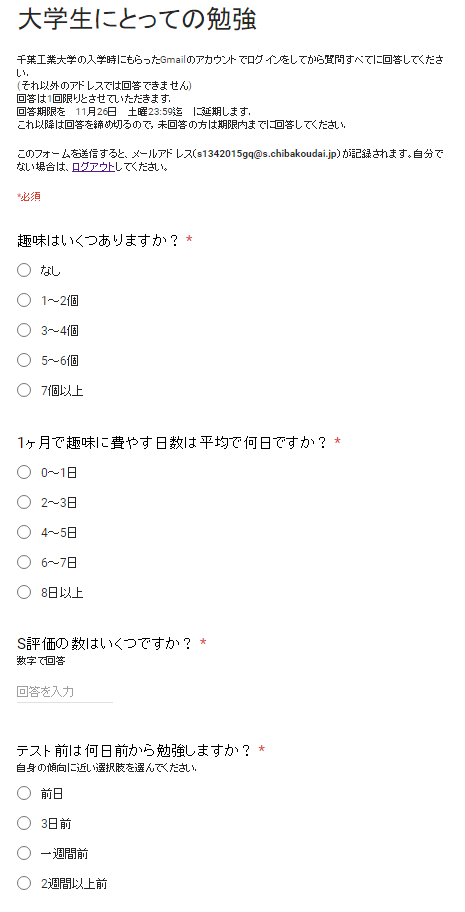
\includegraphics[width=11cm]{forms1.PNG}
\caption{データマイニング入門 アンケート1}\label{サンプル図}
\end{figure}

%図の挿入
\begin{figure}[p]
\centering
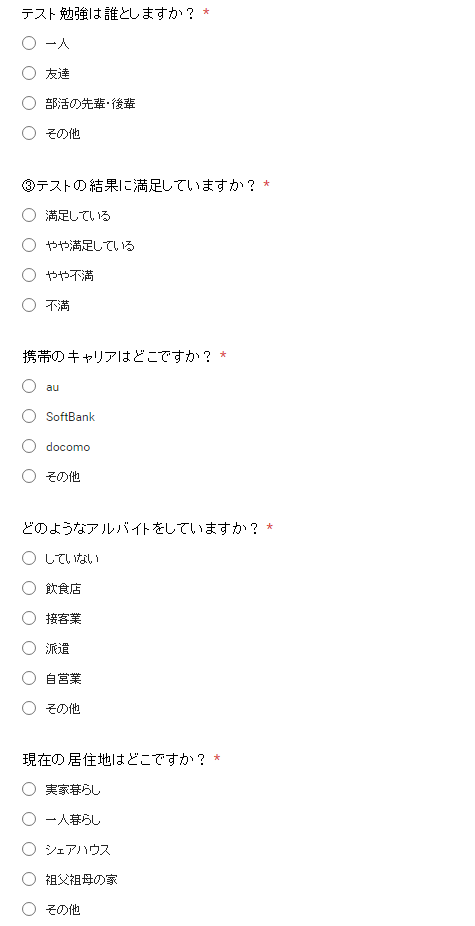
\includegraphics[width=11cm]{forms2.PNG}
\caption{データマイニング入門 アンケート2}\label{サンプル図}
\end{figure}

%図の挿入
\begin{figure}[p]
\centering
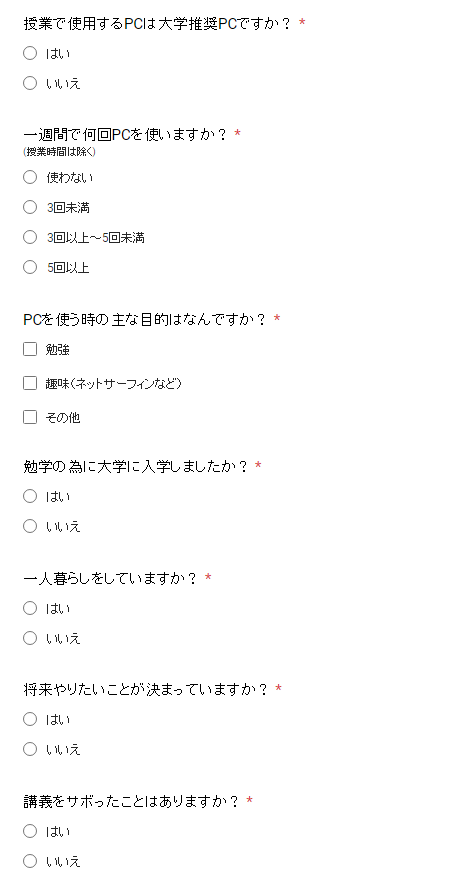
\includegraphics[width=11cm]{forms3.PNG}
\caption{データマイニング入門 アンケート3}\label{サンプル図}
\end{figure}

%図の挿入
\begin{figure}[p]
\centering
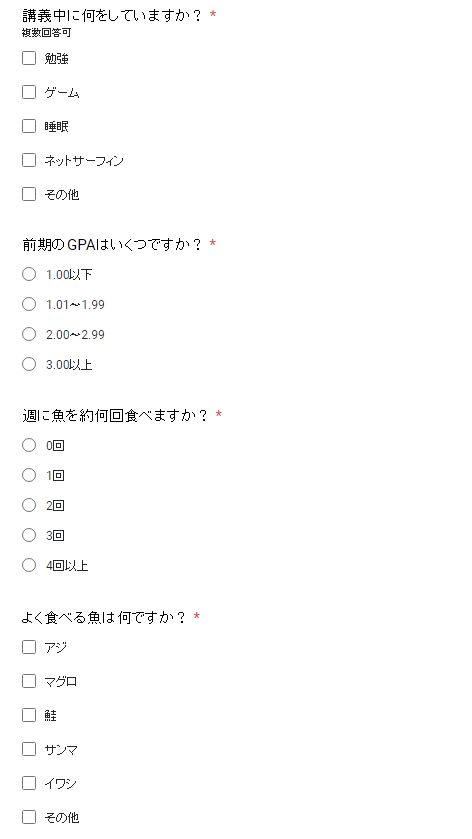
\includegraphics[width=11cm]{forms4.PNG}
\caption{データマイニング入門 アンケート4}\label{サンプル図}
\end{figure}

%図の挿入
\begin{figure}[p]
\centering
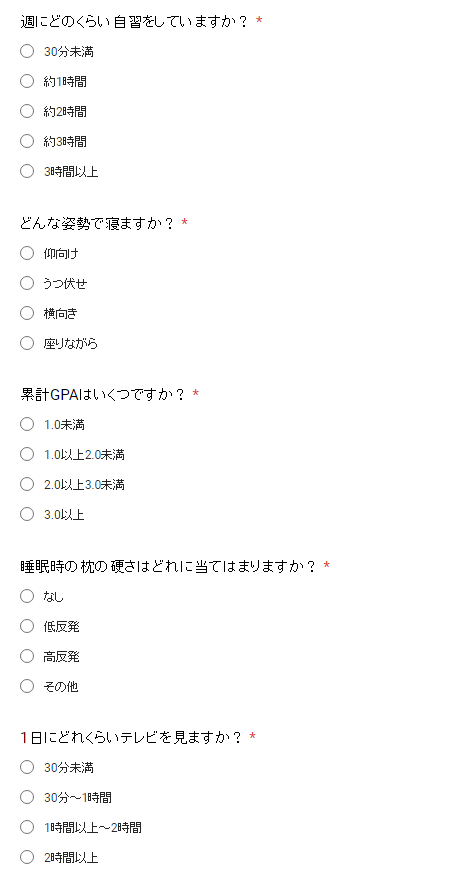
\includegraphics[width=11cm]{forms5.PNG}
\caption{データマイニング入門 アンケート5}\label{サンプル図}
\end{figure}

%図の挿入
\begin{figure}[p]
\centering
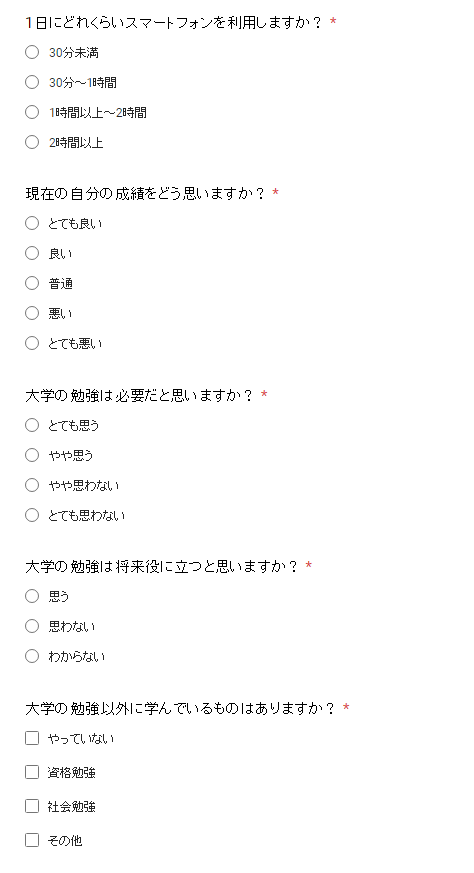
\includegraphics[width=11cm]{forms6.PNG}
\caption{データマイニング入門 アンケート6}\label{サンプル図}
\end{figure}

%図の挿入
\begin{figure}[p]
\centering
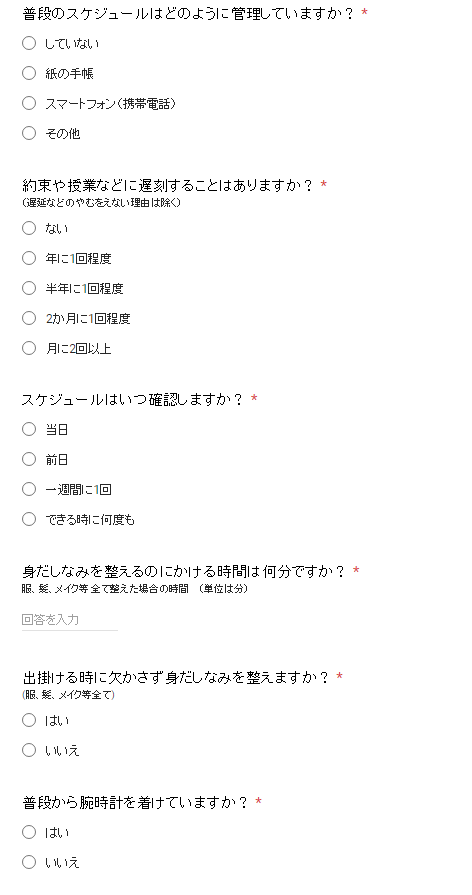
\includegraphics[width=10cm]{forms7.PNG}
\caption{データマイニング入門 アンケート7}\label{サンプル図}
\end{figure}

%図の挿入
\begin{figure}[p]
\centering
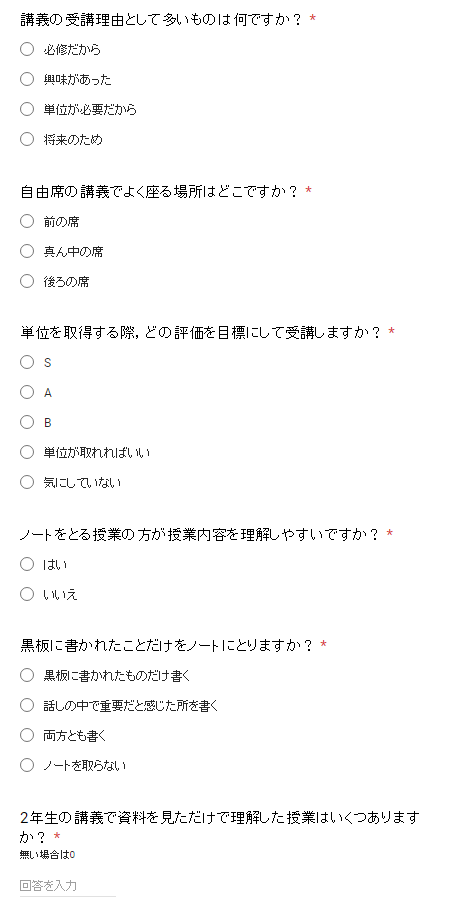
\includegraphics[width=11cm]{forms8.PNG}
\caption{データマイニング入門 アンケート8}\label{サンプル図}
\end{figure}

%図の挿入
\begin{figure}[p]
\centering
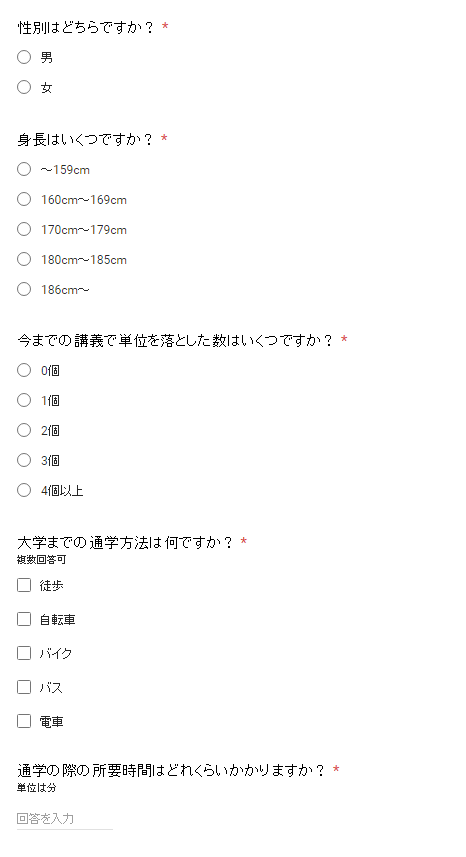
\includegraphics[width=11cm]{forms9.PNG}
\caption{データマイニング入門 アンケート9}\label{サンプル図}
\end{figure}

%図の挿入
\begin{figure}[p]
\centering
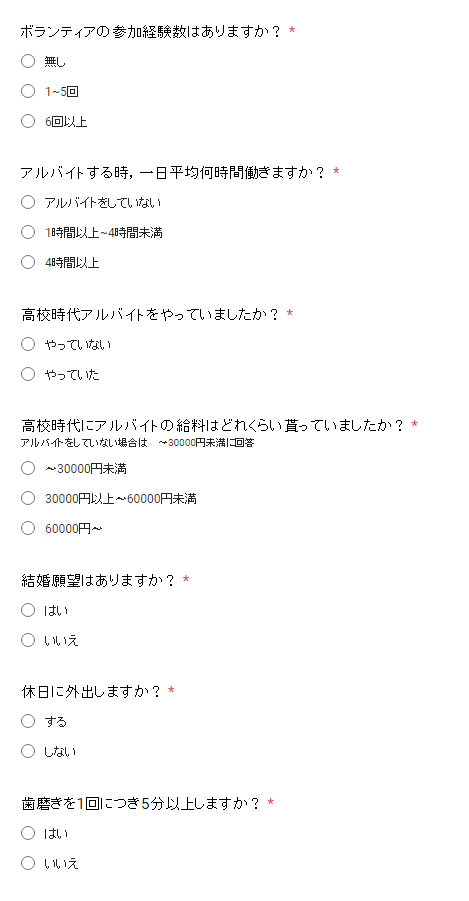
\includegraphics[width=11cm]{forms10.PNG}
\caption{データマイニング入門 アンケート10}\label{サンプル図}
\end{figure}

%図の挿入
\begin{figure}[p]
\centering
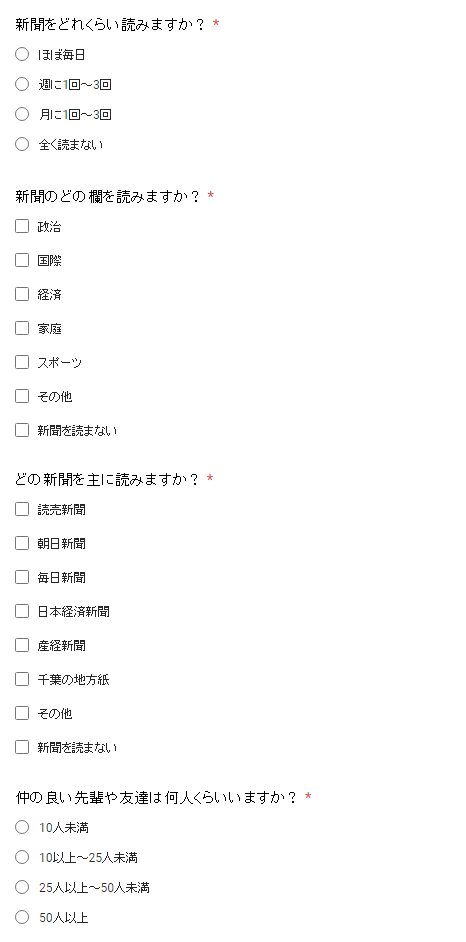
\includegraphics[width=10cm]{forms11.PNG}
\caption{データマイニング入門 アンケート11}\label{サンプル図}
\end{figure}

%図の挿入
\begin{figure}[p]
\centering
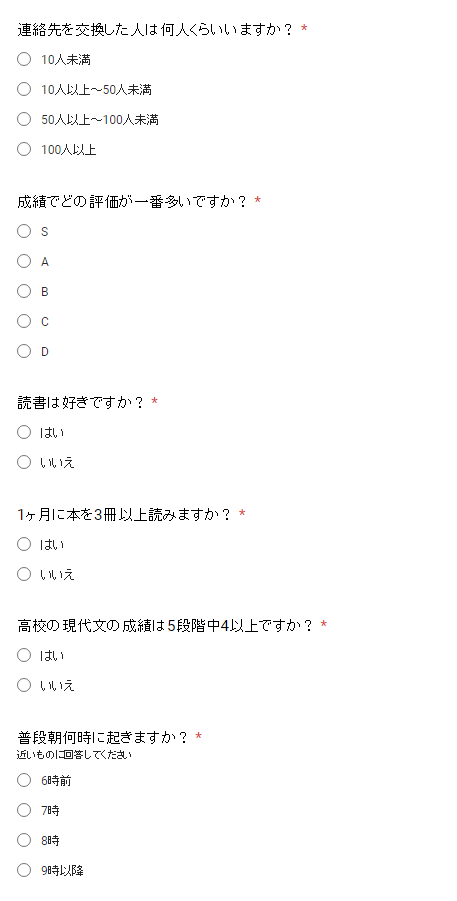
\includegraphics[width=11cm]{forms12.PNG}
\caption{データマイニング入門 アンケート12}\label{サンプル図}
\end{figure}


%図の挿入
\begin{figure}[p]
\centering
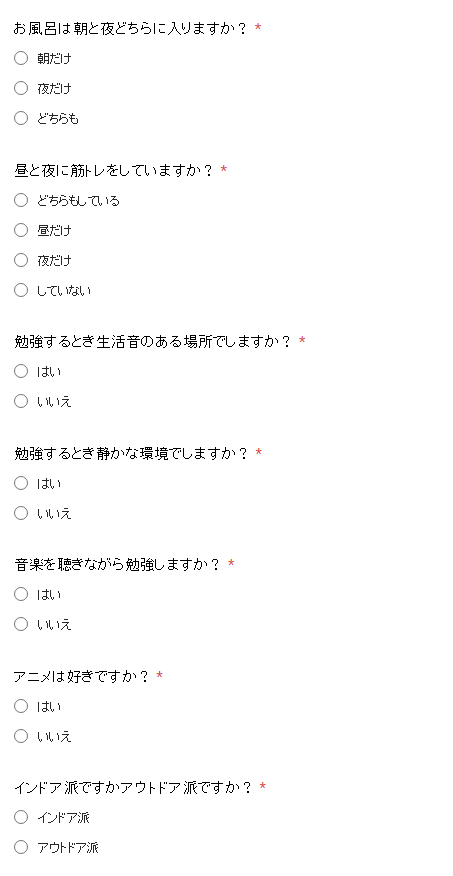
\includegraphics[width=11cm]{forms13.PNG}
\caption{データマイニング入門 アンケート13}\label{サンプル図}
\end{figure}

%図の挿入
\begin{figure}[p]
\centering
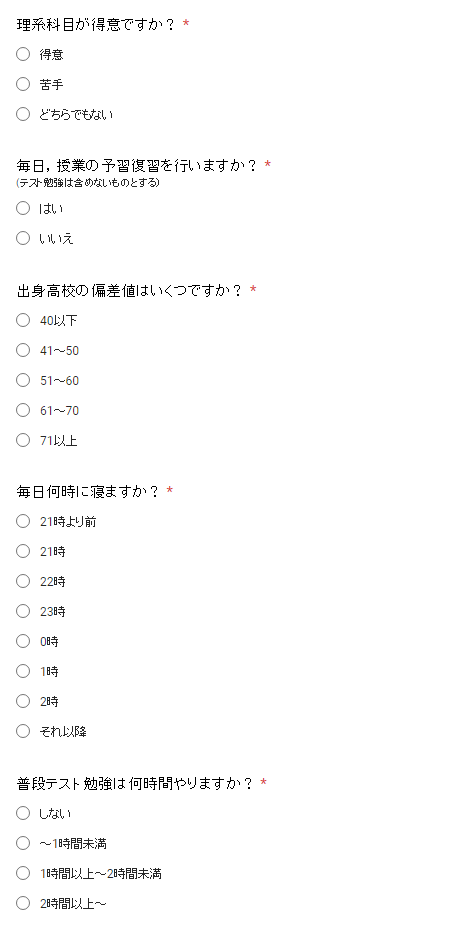
\includegraphics[width=10cm]{forms14.PNG}
\caption{データマイニング入門 アンケート14}\label{サンプル図}
\end{figure}

%図の挿入
\begin{figure}[p]
\centering
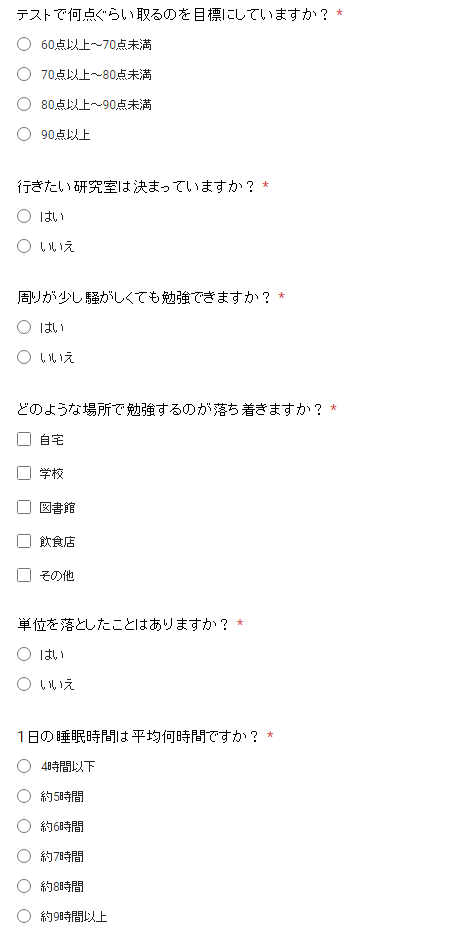
\includegraphics[width=10cm]{forms15.PNG}
\caption{データマイニング入門 アンケート15}\label{サンプル図}
\end{figure}

%図の挿入
\begin{figure}[p]
\centering
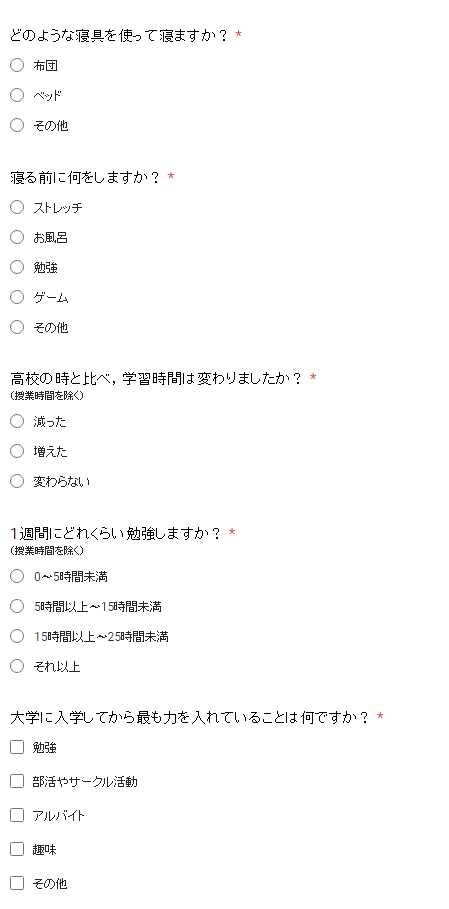
\includegraphics[width=10cm]{forms16.PNG}
\caption{データマイニング入門 アンケート16}\label{サンプル図}
\end{figure}

%図の挿入
\begin{figure}[p]
\centering
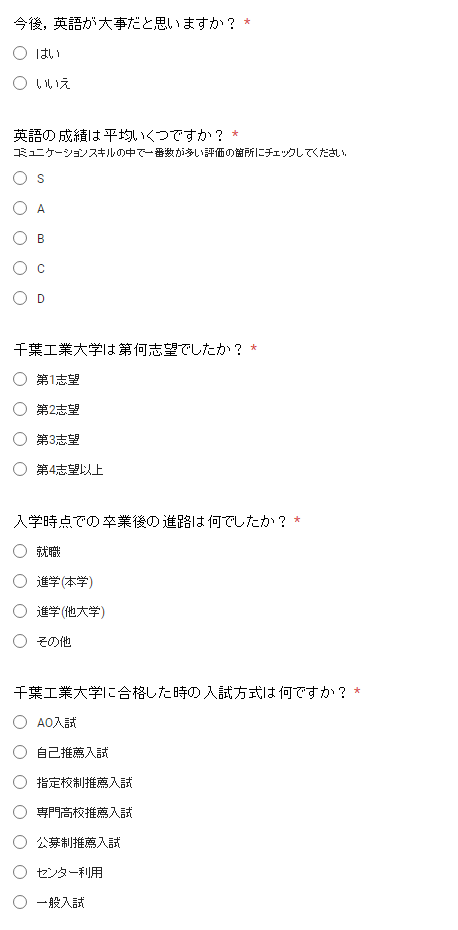
\includegraphics[width=10cm]{forms17.PNG}
\caption{データマイニング入門 アンケート17}\label{サンプル図}
\end{figure}

\newpage

アンケートの回答期限が大学祭と重なってしまったこともあり,期限内に回答してくれた受講者が少なかった.PM本人やPMがグループのメンバーと連絡が取れずアンケートのURLを共有できていなかったというケースもあったため,回答期限を11月26日までに延長した.その結果,119名が回答しデータが集まった.

また,アンケートを取る際に,スプレッドシートを用いて回答者の学績番号と回答日時が記録されるようにした.受講者に回答結果を配布する際には,学籍番号部分を削除することで回答者のプライバシーを守ることができる.
配布したアンケート結果をどの解析手法が有効か各グループで相談しマイニングしてもらう.

スプレッドシートにまとめた回答を以下に図で示す.  \vspace{0.1in} \\*

%図の挿入
\begin{figure}[h]
\centering
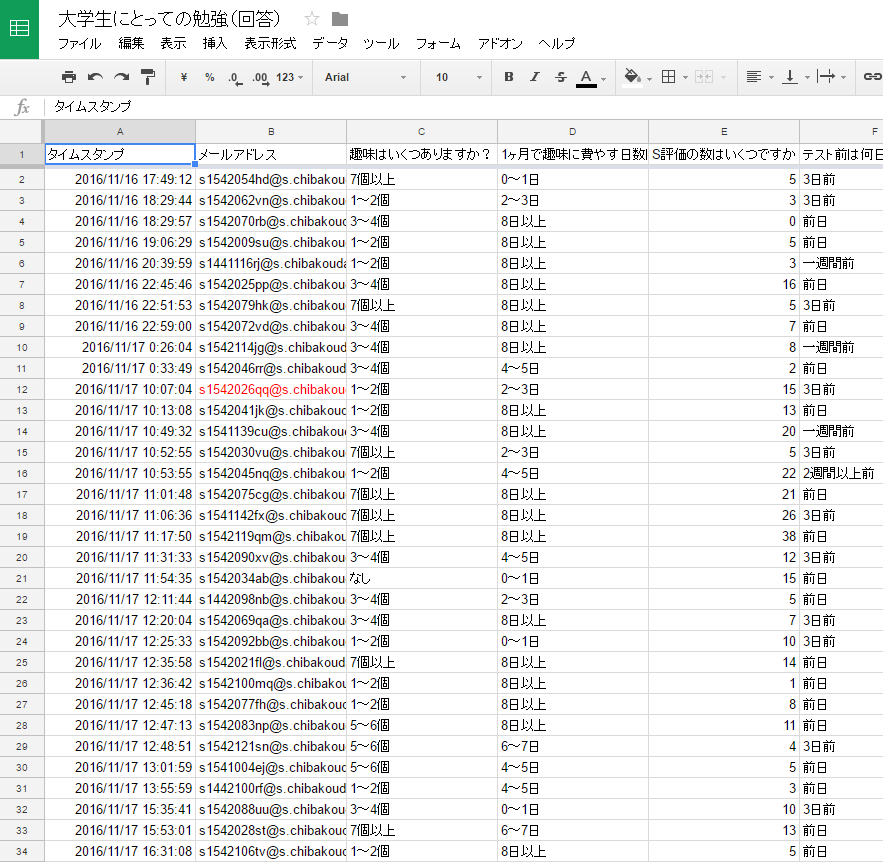
\includegraphics[width=14cm]{sheet.PNG}
\caption{データマイニング入門 アンケート結果}\label{サンプル図}
\end{figure}

\newpage

\begin{description}
 \item[第4週目]\mbox{}\\  \vspace{0.1in} \\*
	配布したアンケートの結果を基に,受講者には自分のグループと全ての質問の結果をデータマイニングしてもらい成果物発表を行った.
グループワークの期間に欠席しており,グループワークには参加できなかったがデータマイニングをしてきた生徒もいたので発表してもらった.
各グループの発表からデータマイニングに使用した解析手法と相関の有無,相関があるグループの一例を以下に記す.  \vspace{0.1in} \\*
\end{description}

\begin{description}
 \item[JABEEコース]\mbox{}\\
\end{description}

\begin{table}[hbtp]
  \caption{JABEEコースのグループと解析手法}
  \label{table:data_type}
  \centering
  \begin{tabular}{|c|c|c|}   \hline
    グループ & 解析手法 & 相関  \\ \hline
    グループ0 & 重回帰分析 & なし \\ \hline
    グループ1 & 重回帰分析 & なし \\ \hline
    グループ2 & ピボットテーブル & あり \\ \hline
    グループ3 & 数量化2類分析 & なし \\ \hline
    グループ4 & 決定木分析,ピボットテーブル & あり \\ \hline
    グループ5 & 決定木分析,ピボットテーブル & あり \\ \hline
    グループ6 & 回帰分析 & なし \\ \hline
    グループ7 & 回帰分析 & なし \\ \hline
    グループ8 & ピボットテーブル & あり \\ \hline
    グループ9 & ピボットテーブル & 不明 \\ \hline
    グループ10 & 回帰分析 & なし \\ \hline
    グループ11 & 回帰分析 & あり \\ \hline
    グループ12 & 不明 & 不明 \\ \hline
    グループ13 & χ2検定 & なし \\ \hline
    グループ14 & 回帰分析 & なし \\ \hline
    グループ15 & 数量化理論2類 & なし \\ \hline
    グループ32 & 数量化理論1類 & あり \\ \hline
  \end{tabular}
\end{table}

\begin{description}
  \item[グループ5] きちんと講義に出席している人は成績が良い人が多いことがわかった.
  \item[グループ11] 優秀な生徒(GPA3.0以上)なほど身だしなみにかける時間が多い.
  \item[グループ32] 寝る前にストレッチをして睡眠時間が7時間かつ就寝時間が22時間の人は成績が良い.
\end{description}

\newpage


\begin{description}
 \item[PMコース]\mbox{}\\
\end{description}

\begin{table}[hbtp]
  \caption{PMコースのグループと解析手法}
  \label{table:data_type}
  \centering
  \begin{tabular}{|c|c|c|}
    \hline
    グループ & 解析手法 & 相関  \\ \hline
    グループ16 & 重回帰分析 & あり \\ \hline
    グループ17 & 決定木分析 & 不明 \\ \hline
    グループ18 & 決定木分析 & 不明 \\ \hline
    グループ19 & 重回帰分析 & あり \\ \hline
    グループ20 & 決定木分析 & 不明 \\ \hline
    グループ21 & ピボットテーブル & あり \\ \hline
    グループ22 & 回帰分析 & なし \\ \hline
    グループ23 & 重回帰分析 & なし \\ \hline
    グループ24 & 重回帰分析 & あり \\ \hline
    グループ25 & 回帰分析 & あり \\ \hline
    グループ26 & 決定木分析 & 不明 \\ \hline
    グループ27 & 回帰分析 & なし \\ \hline
    グループ28 & 決定木分析 & なし \\ \hline
    グループ29 & ピボットテーブル & なし \\ \hline
    グループ30 & 重回帰分析 & なし \\ \hline
    グループ31 & 決定木分析,ピボットテーブル & あり \\ \hline
  \end{tabular}
\end{table}

\begin{description}
  \item[グループ19] 交友関係が広い人は成績が良い人が多い.
  \item[グループ25] テストで高得点を取る人ほどテスト勉強の時間が多い.
  \item[グループ31] 英語の成績が高い人はGPAも高い.  \vspace{0.1in} \\*
\end{description}

1つの解析手法で相関が見られなかったため,違う解析手法を用いてデータマイニングを行ったグループは解析手法を2つ記載している.また,解析手法に誤りがあったグループや解析手法を用いずに発表したグループは不明と記載している.


\newpage

データマイニング入門でアクティブラーニングを取り入れ,成果物発表を行った.解析手法で最も多く使用されたのは回帰分析とピポットテーブルであった.回帰分析はRとExcelのどちらでも簡単に出来,講義内で多く使用したことから学生が選んだと考えられる.

相関のあったグループは12グループ,無いグループは15グループだった.相関の無いグループの方が多いことから相関がありそうな質問を考える事は難しいことがわかる.相関があるグループで面白い結果が出たグループは少なかったが,とても良くマイニングをしているグループがあったので一部紹介する.  \vspace{0.1in} \\*
グループ32は数ある質問から有意Fの値が高い質問データだけを絞り込み,信頼性の高いデータをさらにマイニングするという方法で相関を出していた.

結果として,発表から有意な結果はあまり得られなかった.しかしながら,学習者自身が大学生にとっての勉強と相関があるかを考えて質問を作ったことで,学習者の能動的な学習への参加を取り入れた能力の育成をすることができた.成果物発表の際,考察を交え発表してもらったが,「質問をより具体的な物にする」という意見が多かった.質問の質を高めるためにもグループで話し合う時間や解析手法の例を事前に紹介しておくことでこのような問題を回避できると考える.

\section{考察}
今回4 週間でグループワークを行ったが,質問を考える段階からどのような結果が得られるのかを想定して計画していく必要があった.また,各週の講義内でグループワークを割り当てるよう設計するとさらに効果的なアクティブラーニングを行うことができるだろう.







\bibliographystyle{junsrt}
\bibliography{biblio}%「biblio.bib」というファイルが必要.

\chapter*{謝辞}\addcontentsline{toc}{chapter}{謝辞}
本研究を進めるにあたり,矢吹研究室矢吹太朗准教授には,多くの時間をご指導にさいて頂きました.また矢吹研究室の皆様には,多くの知識や示唆を頂きました.協力していただい皆様に感謝の気持ちと御礼を申し上げます.



\end{document}
